\chapter{SN~1987A}\label{chp:chp5}

\begin{flushright}
  {\em QUOTE GOES HERE }\\

\ \

\normalsize
{AUTHOR}  
\end{flushright}

\section{Spectral Observations of SN 1987A}
\label{spectra}

SN~1987A has been the most intensively observed supernova in history, with 
a wealth of both spectral and photometric data available to model.  From 
the archives of a number of different telescopes we have collated optical 
spectra acquired over a wide range of epochs.  At the earlier epochs we 
use spectra obtained with the Anglo-Australian Telescope (AAT) and Cerro 
Tololo Inter-American Observatory (CTIO) and at later epochs we 
use spectra from the archives of the Hubble Space Telescope (HST) and Very 
Large Telescope (VLT).  An explosion date of 23 February 1987 is adopted 
throughout and epochs are measured relative to this date.  Full details of 
all observations may be found in Table \ref{tb:data}. The spectral 
resolutions of the grating spectrograph observations are listed in 
column~7, while column~8 lists the spectral resolving powers of the 
echelle spectrograph observations.

Wavelength ranges encompassing the H$\alpha\ $ line and [O~{\sc i}] 
$\lambda$6300,6363~\AA\ doublet were selected in order to trace their 
evolution from day 524, near the time of the first indications of dust 
formation (Wooden et al. 1993) to day 8020, near the current era. Optical 
spectroscopy obtained at the AAT using the Faint Object Red Spectrogaph 
(FORS) during the first two years after outburst was kindly supplied by Dr Raylee 
Stathakis \citep{Spyromilio1991, Spyromilio1993a, Hanuschik1993}.

\begin{table*}
	\begin{minipage}{180mm}
	\caption{Details of the archival data for SN 1987A}
	\label{tb:data}
  	\begin{tabular}{@{} ccccccccl @{}}
    	\hline
	Date & Age & Telescope  & Inst & $\lambda_{min}$ & $\lambda_{max}$ & Res. & Res. Power & Reference \\
	& (days) & & &(\AA) & (\AA)& (\AA)\\
	\hline
31 Jul 1988 & 524 & AAT & FORS & 5500 & 10190 & 20 & & \citet{Spyromilio1991} \\
26 Oct 1988 & 611 & AAT & UCLES & 6011 & 7336 &  & 30000 & \citet{Hanuschik1993, Spyromilio1993a}\\
27 Dec 1988 & 673 & AAT & UCLES & 5702 & 10190 &  & 30000 & \citet{Hanuschik1993, Spyromilio1993a}\\
06 Feb 1989 & 714 & CTIO-1.5m & Cass. & 6420 & 10380 & 16 & & \citet{Phillips1990}\\
09 May 1989 & 806 & CTIO-1.5m & Cass. & 6430 & 10330 & 16 & & \citet{Phillips1990}\\
30 Mar 1992 & 1862 & HST & STIS & 4569 & 6818 & 4.4 &  & \citet{Wang1996}\\
14 Mar 1993 & 2211 & HST & STIS & 4569 & 6818 & 4.4 &  & \citet{Wang1996}\\
07 Jan 1995 & 2875 & HST & STIS & 4569 & 6818 & 4.4 &  & \citet{Chugai1997}\\
23 Sep 1996 & 3500 & HST & STIS & 4569 & 6818 & 4.4 &  \\
05 Jan 1997 & 3604 & HST & STIS & 4569 & 6818 & 4.4 &  \\
10 Dec 2000 & 5039 & VLT & UVES & 4760 & 6840 &  & 50000 & \citet{Groeningsson2006, Groeningsson2007}\\
06 Oct 2002 & 5704 & VLT & UVES & 4760 & 6840 &  & 50000 & \citet{Groeningsson2006, Groeningsson2007, Groningsson2008}\\
21 Mar 2005 & 6601 & VLT & UVES & 4760 & 6840 &  & 50000 &\citet{Groeningsson2006, Groeningsson2007}\\
23 Oct 2007 & 7547 & VLT & UVES & 4760 & 6840 &  & 50000 & \citet{Groeningsson2007}\\
07 Feb 2009 & 8020 & VLT & UVES & 4800 & 6800 &  & 50000 & \citet{Tziamtzis2010}\\
    \hline
  \end{tabular}
\end{minipage}
\end{table*}


The evolution of the H$\alpha$ line profile is presented in Figures 
\ref{Ha_evol_early} and \ref{Ha_evol_late}.  At later epochs, the broad 
profile emitted by the ejecta becomes contaminated by narrow line emission 
from the equatorial ring.  These lines have been removed for the purposes 
of modelling the broad line. A continuum fit has been subtracted from each 
spectrum and a velocity correction has been applied for a recession 
velocity of 287 km~s$^{-1}$ \citep{Groningsson2008}.

\begin{table*}
	\begin{minipage}{180mm}
	\caption{Details of the parameters used for the best fitting smooth models with grain radius $a=0.35\mu$m.}
	\label{smooth1}
	\begin{center}
  	\begin{tabular}{@{} ccccccccccccl @{}}
    	\hline
 & day & $V_{max}$ & $R_{in}/R_{out}$ & $\beta$ & $M_{dust}$ & $a$ & $R_{out}$ & $R_{in}$ & doublet ratio & $\tau_{H\alpha}$ & $\tau_V$  & Figure No. \\
	&& (km~s$^{-1} $) & & & ($M_{\odot}$) & ($\mu$m) & (cm) & (cm) & [O~{\sc i}] \\
	\hline
H$\alpha$ & 714 & 3250 & 0.25 & 1.2 & 2.50E-05 & 0.35 & 2.00E+16 & 5.01E+15 & & 0.61 & 1.23 &  Fig. \ref{d714bf}\\
H$\alpha$ & 806 & 4500 & 0.25 & 1.8 & 3.00E-05 & 0.35 & 3.13E+16 & 7.83E+15 & & 0.30 & 0.60 &  Fig. \ref{d806bf}\\
H$\alpha$ & 1862 & 8500 & 0.15 & 1.9 & 6.00E-04 & 0.35 & 1.37E+17 & 2.05E+16 & & 0.35 & 0.70 &  Fig. \ref{d1862_3604}\\
H$\alpha$ & 2875 & 9500 & 0.14 & 1.9 & 1.80E-03 & 0.35 & 2.36E+17 & 3.30E+16 & & 0.36 & 0.72 &  Fig. \ref{d1862_3604}\\
H$\alpha$ & 3604 & 10250 & 0.13 & 1.9 & 5.00E-03 & 0.35 & 3.19E+17 & 4.15E+16 & & 0.55 & 1.10 &  Fig. \ref{d1862_3604}\\ \relax
[O~{\sc i}]  & 714 & 5000 & 0.17 & 2.8 & 9.50E-05 & 0.35 & 3.08E+16 & 5.24E+15 & 2.9 & 1.09 & 2.19 & Fig. \ref{d714bf}\\ \relax
[O~{\sc i}]  & 806 & 6000 & 0.15 & 2.7 & 1.60E-04 & 0.35 & 4.18E+16 & 6.27E+15 & 2.7 & 0.97 & 1.95 & Fig. \ref{d806bf} \\
    \hline
  \end{tabular}
  \end{center}
\end{minipage}
\end{table*}

\section{Modelling SN~1987A}
\label{results}

\begin{figure}
\begin{center}
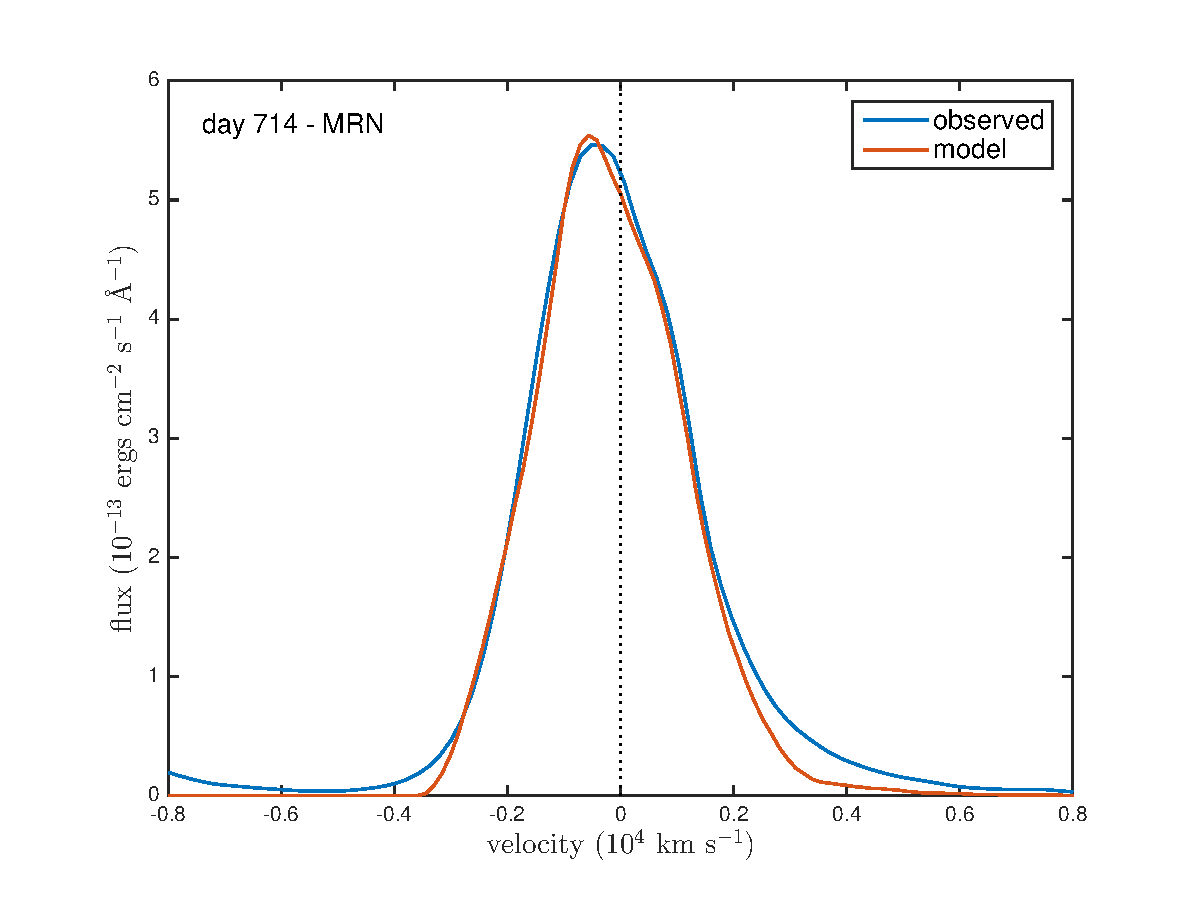
\includegraphics[trim =37 10 45 15,clip=true,scale=0.51]{chapters/chapter5/images/smooth/d714Ha_smooth_amC_MRN}
\caption{Conservative dust mass fit to the day 714 H$\alpha$ line of SN~1987A illustrating the 
underestimation of the red scattering wing for small grain sizes.  Model 
parameters are the same as the conservative fit to day 714 except for the 
grain size distribution and dust mass:  $V_{max}=3250$ km~s$^{-1}$, 
$R_{in}/R_{out}$=0.25, $\beta = 1.2$, $M_{dust}=8.0 \times 10^{-6} 
M_{\odot}$, $a_{min}=0.005 \mu$m, $a_{max}=0.25 \mu$m and $n(a) \propto 
a^{-3.5}$.}
\label{MRN}
\end{center}
\end{figure}

\begin{figure*}
\begin{center}
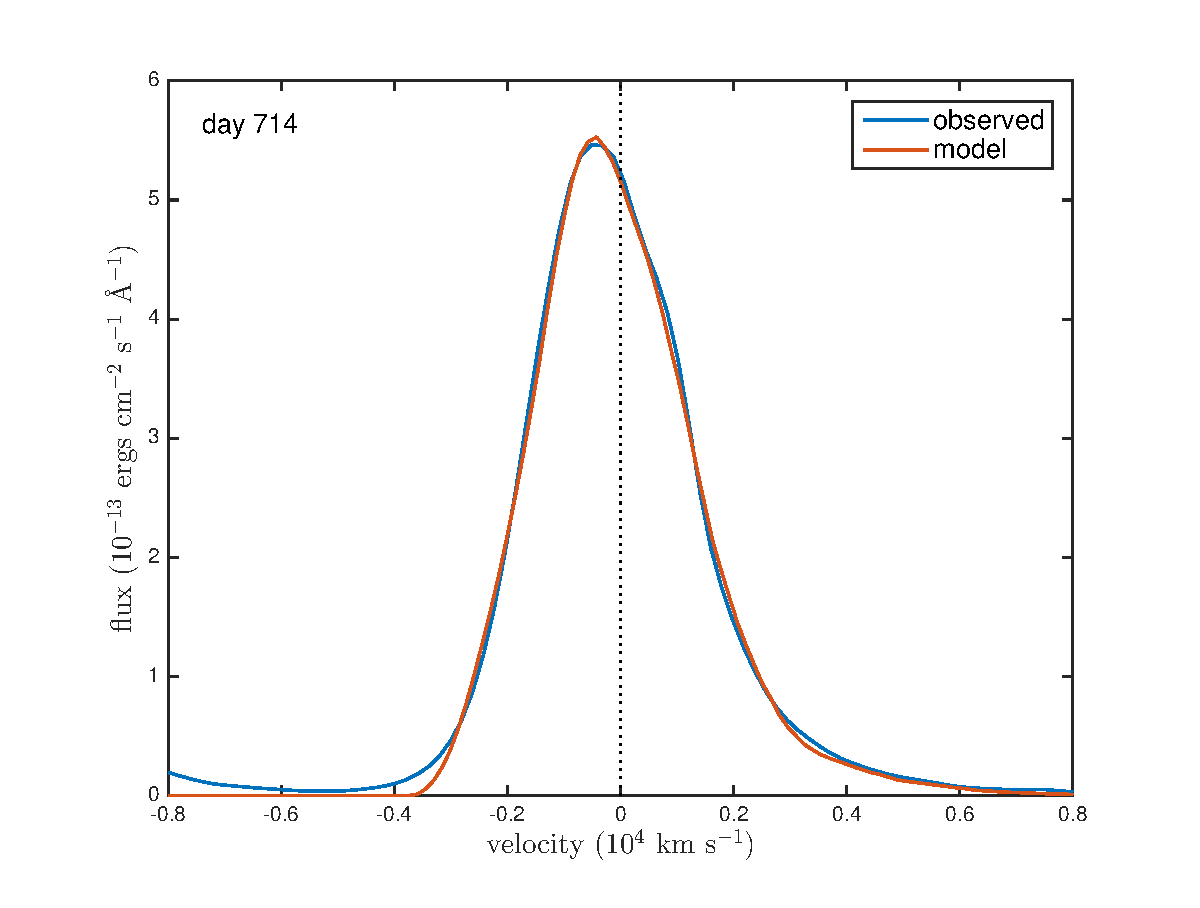
\includegraphics[trim =37 10 45 15,clip=true,scale=0.51]{chapters/chapter5/images/smooth/best_fit/d714Ha}
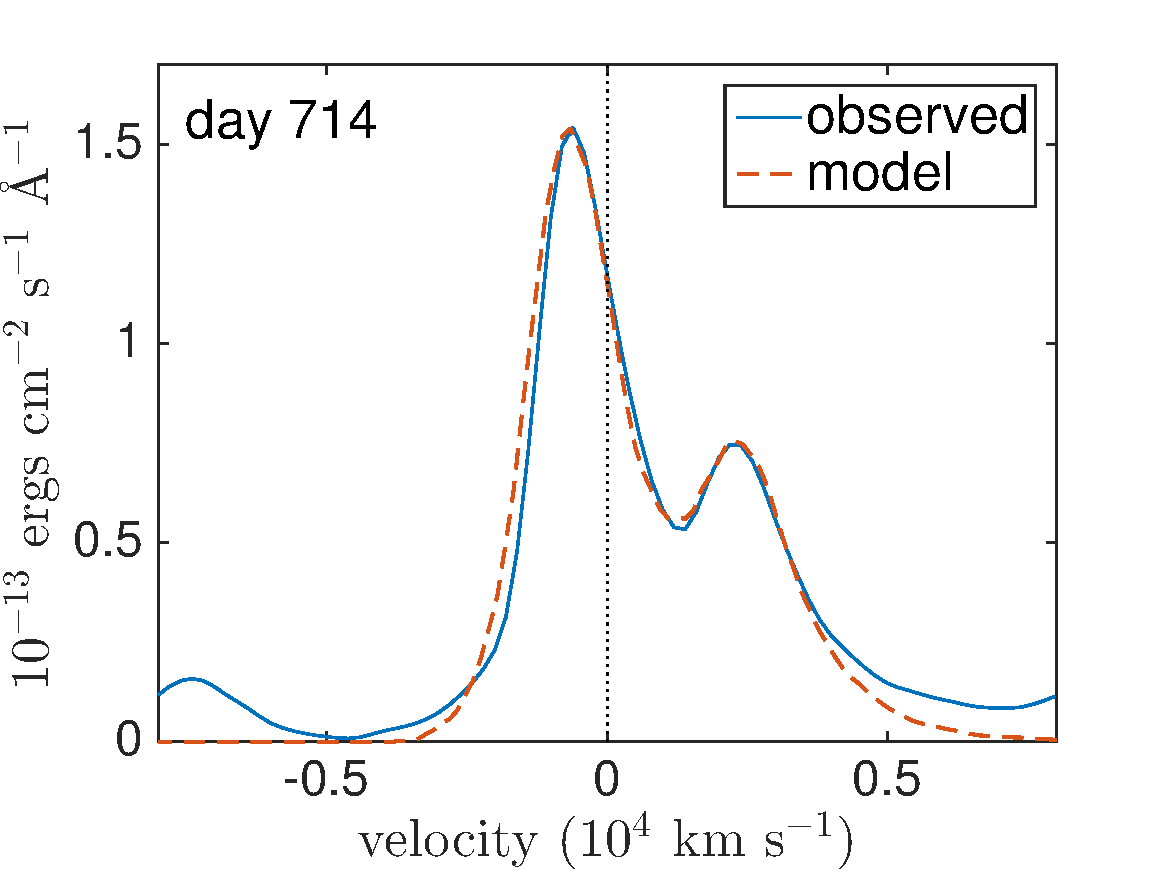
\includegraphics[trim =37 10 45 15,clip=true,scale=0.51]{chapters/chapter5/images/smooth/best_fit/d714OI}
\caption{Best smooth fit to the day 714 H$\alpha$ line (left) and 
[O~{\sc i}] $\lambda$6300,6363~\AA\ doublet (right) as per parameters 
detailed in Table \ref{smooth1}.}
\label{d714bf}
\end{center}
\end{figure*}
\begin{figure*}
\begin{center}
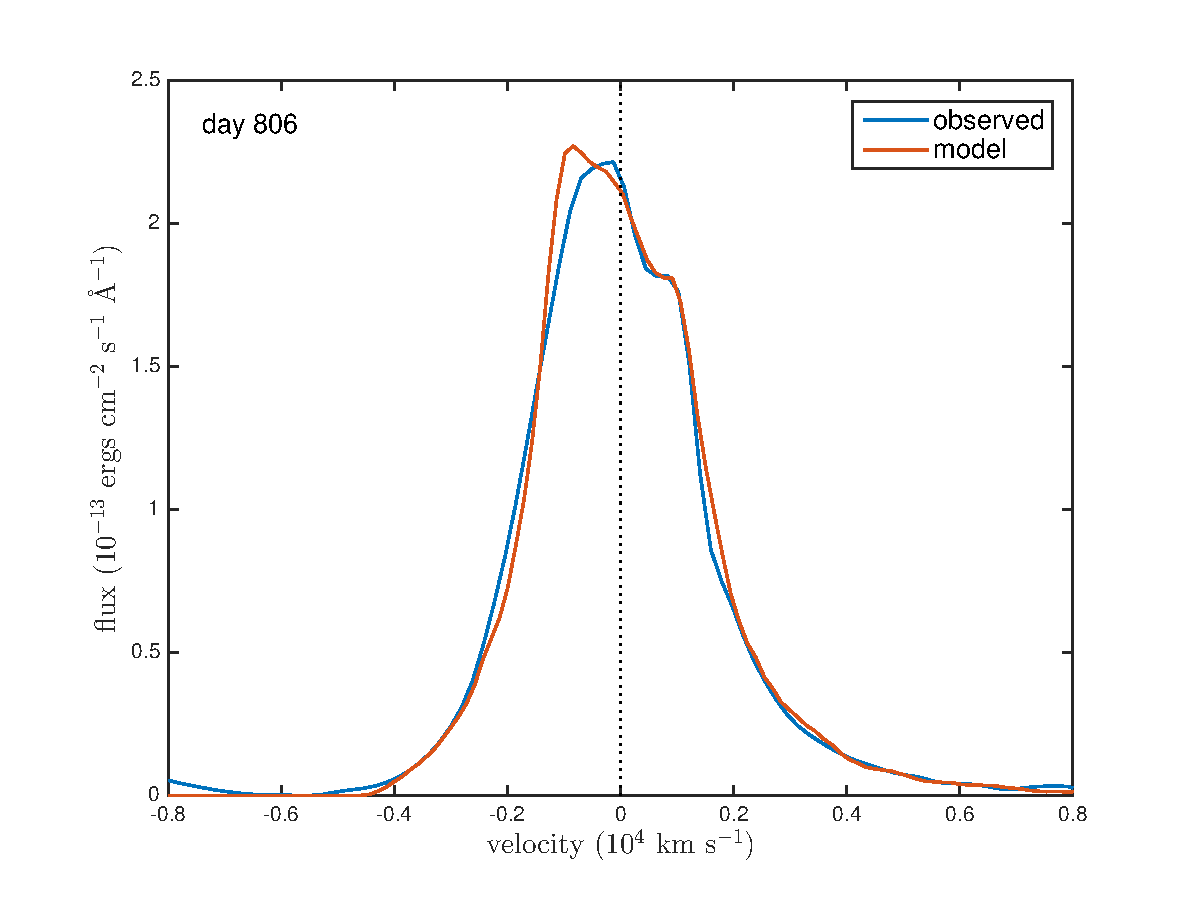
\includegraphics[trim =37 10 45 15,clip=true,scale=0.51]{chapters/chapter5/images/smooth/best_fit/d806Ha}
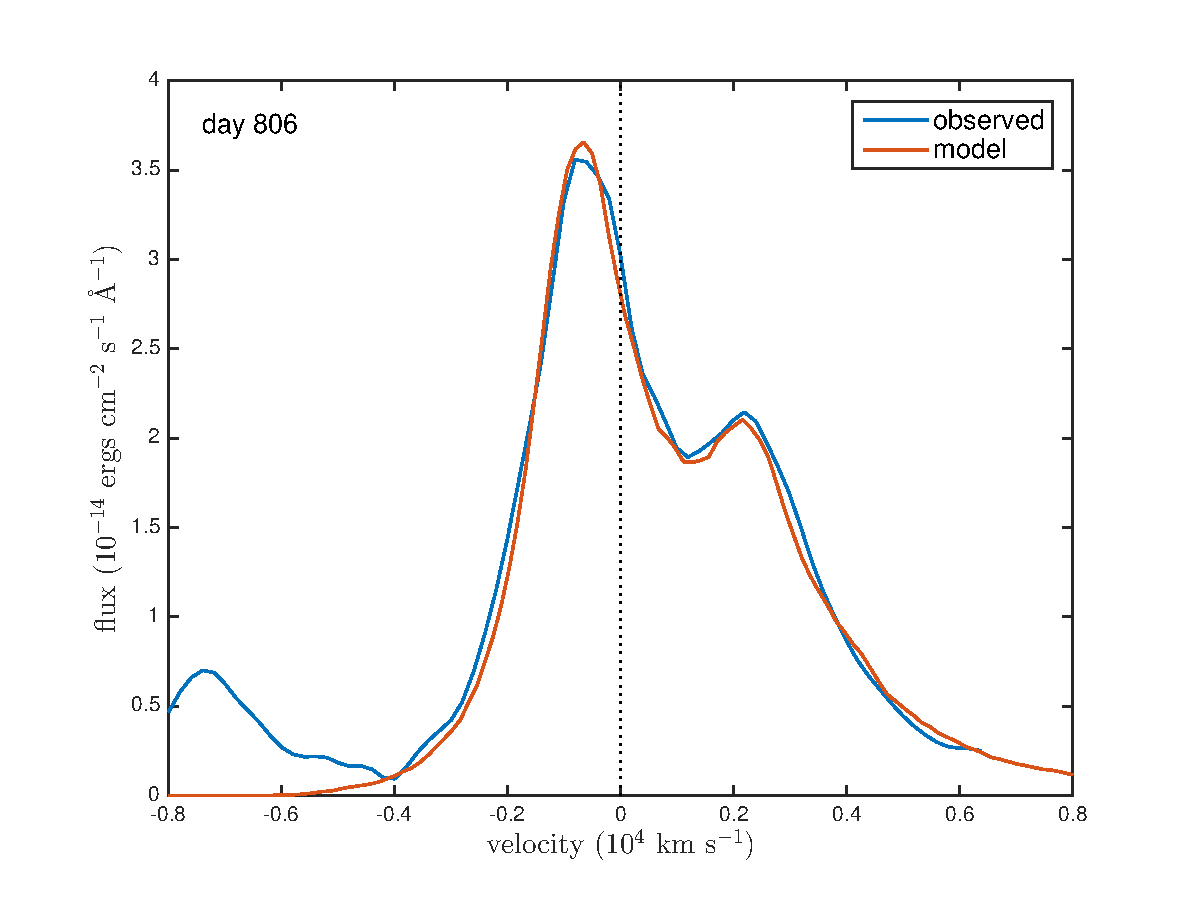
\includegraphics[trim =37 10 45 15,clip=true,scale=0.51]{chapters/chapter5/images/smooth/best_fit/d806OI}
\caption{Best smooth fit to the day 806 H$\alpha$ line (left) and the 
[O~{\sc i}] $\lambda$6300,6363~\AA\ doublet (right) as per parameters 
detailed in Table \ref{smooth1}.}
\label{d806bf}
\end{center}
\end{figure*}


We model the H$\alpha$ line of SN~1987A at days 714, 806, 1862, 2875 and 3604 and the 
[O~{\sc i}] $\lambda$6300,6363~\AA\ doublet at days 714 and 806. After this 
epoch the profile begins to become dominated by emission from the reverse shock 
and the structure of the emitting region may no longer be approximated by 
a single shell model as we do here \citep{Fransson2013}.  We continue to adopt a velocity profile $V(r) = 
\frac{V_{max}}{R_{max}}r$ and treat the variable parameters listed in 
Section \ref{ps}.  Whilst the albedo and optical depth are not varied 
directly, they are altered by adjusting the dust mass, $M_{dust}$, and the 
grain size, $a$, which will together determine the albedo and optical 
depth via a Mie scattering approximation and the optical properties of the 
dust.

In all models, the ejecta occupies a shell with inner radius $R_{in}$ and 
outer radius $R_{out}$.  Packets are emitted according to a smooth density 
profile assuming recombination such that $i(r) \propto \rho(r)^2 \propto 
r^{-2\beta}$.  Initially the dust is considered to have a smooth density 
distribution and is assumed to be coupled to the gas to follow the same 
radial profile.  A clumped distribution of dust is considered later (see 
Section \ref{clumped_models}).  We do not include electron scattering in 
these models since we find that the electron scattering optical depth is not high enough to affect the line 
profiles in any discernible fashion \textit{references}.




There is rarely a unique set of parameters that best fit the data.  However, the 
majority of the parameters of interest can be well constrained by our 
modelling by considering different elements of the shape of the profile.  In particular, by constructing good fits to 
the data using both conservative and optimistic estimates of the grain 
size, credible lower and upper bounds on the possible dust mass formed 
within the ejecta may be derived.  We present here
reasonable fits to the data obtained using both small and large values of the grain radius $a$, since 
it is the grain size which has the most significant effect on the overall 
dust mass required to reproduce the profile (see Section \ref{params}).  
We use pure amorphous carbon dust and use the optical 
constants from the BE sample presented in \citet{Zubko1996}.  Previous SED
modelling of SN~1987A has limited the fraction of silicates present in the dusty 
medium to a maximum of 15\% \citep{Ercolano2007,Wesson2015}. Amorphous 
carbon is the most conservative choice of grain type since the inclusion of even a small 
fraction of silicates increases the dust mass required.

For each profile, the maximum velocity is identified from the data as the 
point where the line vanishes on the blue side.  The equivalent point on 
the red side is indeterminate from observations due to the effects of 
dust scattering.  Similarly, the ``corner'' of the flat topped section of the 
profile on the blue side allows the minimum velocity at radius $R_{in}$ to be 
ascertained. As discussed in Section \ref{params}, this allows the ratio 
of the inner and outer radii of the supernova ejecta to be determined since 
$R_{in}/R_{out}=V_{min}/V_{max}$.  The outer radius is calculated from the 
epoch and maximum velocity.

The only parameters that then remain to be determined are the exponent of 
the density profile $\beta$, the mean grain size radius and the total dust mass.  The shape 
of the blue wing is solely a product of the density profile and the dust 
mass; the height and shape of the red wing is a product of these and also 
of the scattering efficiency of the grains (the albedo $\omega$); and the 
extent and shape of the asymmetry in the flat-topped portion of the 
profile is a result of only the total dust optical depth determined by the 
dust mass and the grain size.  By iterating over these three parameters 
therefore, an excellent fit to the data can usually be obtained.

Models are produced in the same manner for the [O~{\sc i}] 
$\lambda$6300,6363~\AA\ doublet as for a single line, with each component 
of the doublet being modelled independently and the resulting profiles 
added according to a specified ratio.  Although the theoretical intrinsic flux ratio 
is 3.1 for optically thin emission, the actual ratio between the two components can be 
affected by self-absorption (\textit{reference}) and we therefore 
left it as a free parameter.  [O~{\sc i}] 
$\lambda$6300,6363~\AA\ exhibits a clear blueshift as early as day 611 
and provides another diagnostic for determining the dust mass.  By day 1862 
the doublet is no longer strong enough to usefully 
modelled (see Figure \ref{Ha_evol_early}).


\begin{table*}
	\begin{minipage}{180mm}
	\caption{Details of the parameters used for the best fitting clumped models with $a=0.6\mu$m.}
	\label{clumped1}
	\begin{center}
  	\begin{tabular}{@{} ccccccccccccl @{}}
    	\hline
 & day & $V_{max}$ & $R_{in}/R_{out}$ & $\beta$ & $M_{dust}$ & $a$ & $R_{out}$ & $R_{in}$ &  doublet ratio & $\tau_{H\alpha}$ & $\tau_V$  & Figure No. \\
	&& (km~s$^{-1} $) & & & ($M_{\odot}$) & ($\mu$m) & (cm) & (cm)  \\
	\hline
H$\alpha$ & 714 & 3250 & 0.25 & 1.2 & 7.00E-05 & 0.6 & 2.00E+16 & 5.01E+15 & & 0.87 & 1.74 & Fig. \ref{d714_c} \\
H$\alpha$ & 806 & 4250 & 0.25 & 1.9 & 1.00E-04 & 0.6 & 2.96E+16 & 7.40E+15 & & 0.56 & 1.12 & Fig. \ref{d806_c}\\
H$\alpha$ & 1862 & 8500 & 0.14 & 1.9 & 1.65E-03 & 0.6 & 1.37E+17 & 1.91E+16 & & 0.48 & 0.96 & Fig. \ref{d1862_3604_c}\\
H$\alpha$ & 2875 & 9500 & 0.12 & 2 & 1.00E-02 & 0.6 & 2.36E+17 & 2.83E+16 & & 0.96 & 1.93 & Fig. \ref{d1862_3604_c}\\
H$\alpha$ & 3604 & 10250 & 0.12 & 2 & 2.30E-02 & 0.6 & 3.19E+17 & 3.83E+16 & & 1.21 & 2.42 & Fig. \ref{d1862_3604_c}\\ \relax
[O~{\sc i}]  & 714 & 5000 & 0.17 & 2.8 & 2.70E-04 & 0.6 & 3.08E+16 & 5.24E+15 & 2.6 &  1.02 & 2.03 & Fig. \ref{d714_c}\\ \relax
[O~{\sc i}]  & 806 & 6000 & 0.15 & 2.7 & 6.00E-04 & 0.6 & 4.18E+16 & 6.27E+15 & 2.4 & 1.66 & 3.32 & Fig. \ref{d806_c}\\
    \hline
  \end{tabular}
  \end{center}
\end{minipage}
\end{table*}


\begin{figure*}
\begin{center}
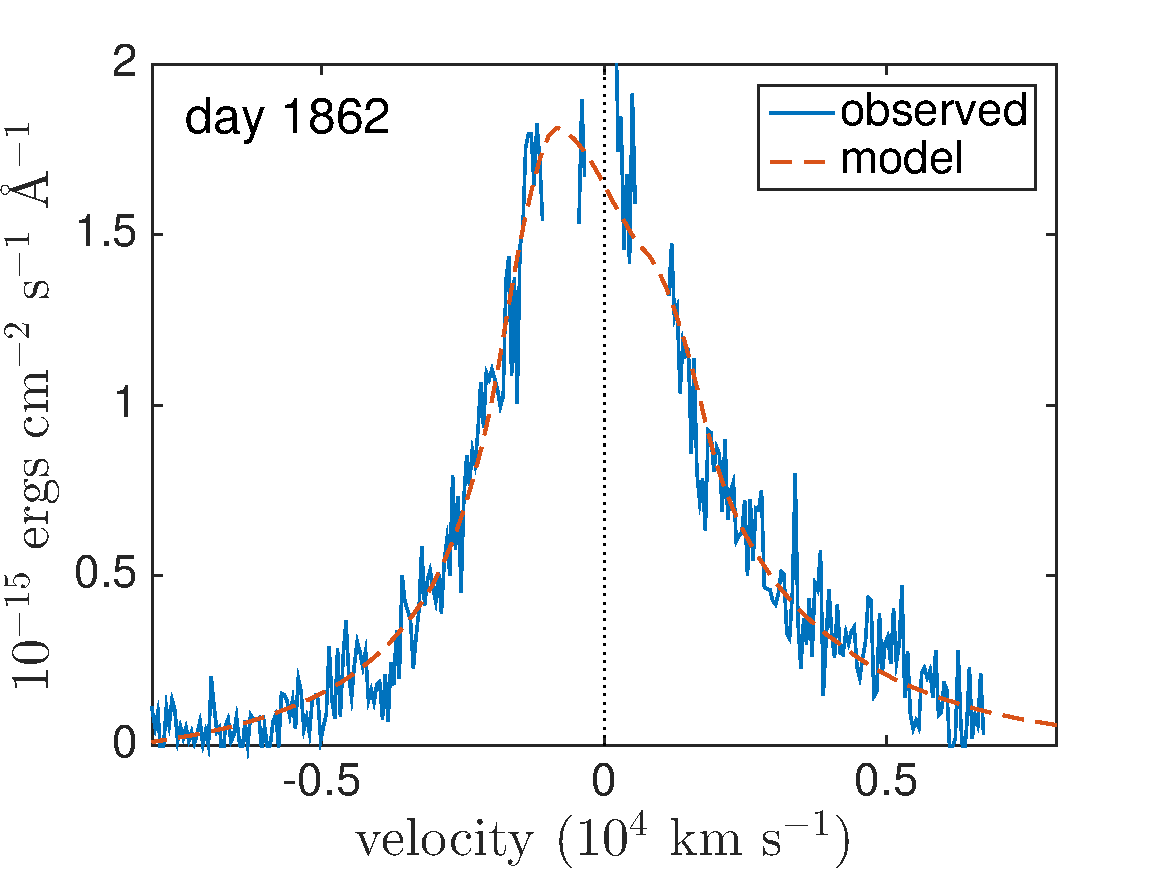
\includegraphics[trim =37 10 45 15,clip=true,scale=0.35]{chapters/chapter5/images/smooth/best_fit/d1862Ha}
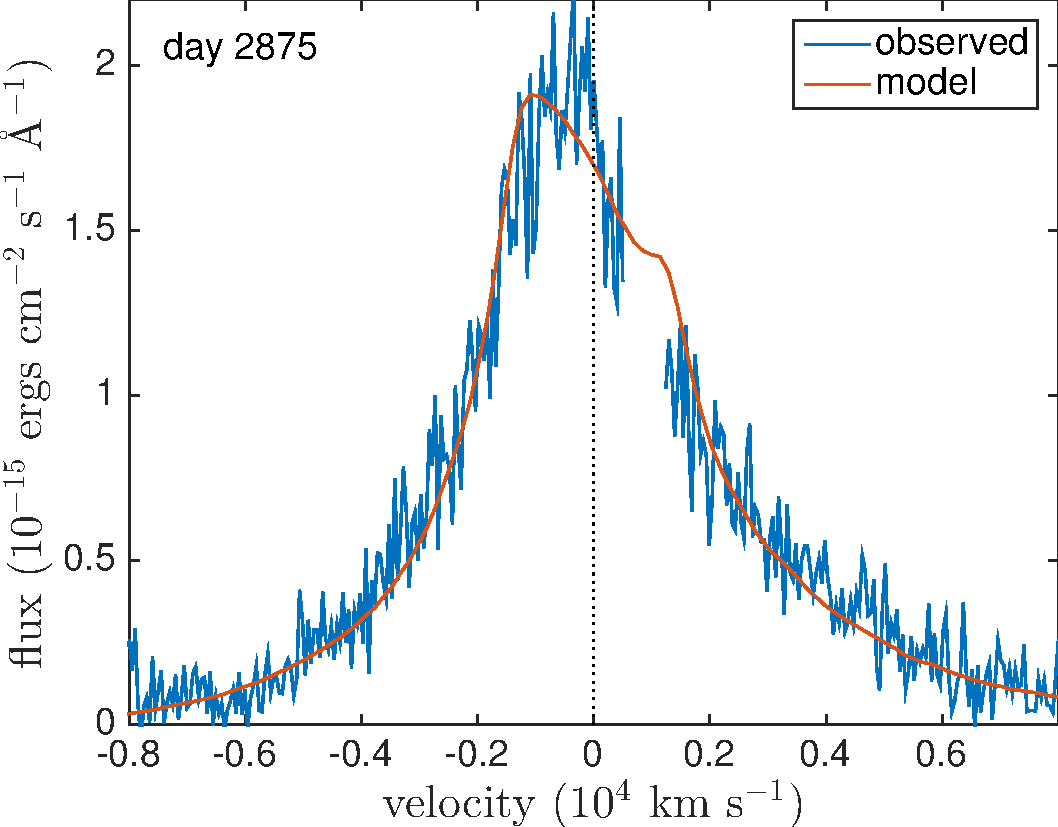
\includegraphics[trim =55 10 45 15,clip=true,scale=0.35]{chapters/chapter5/images/smooth/best_fit/d2875Ha}
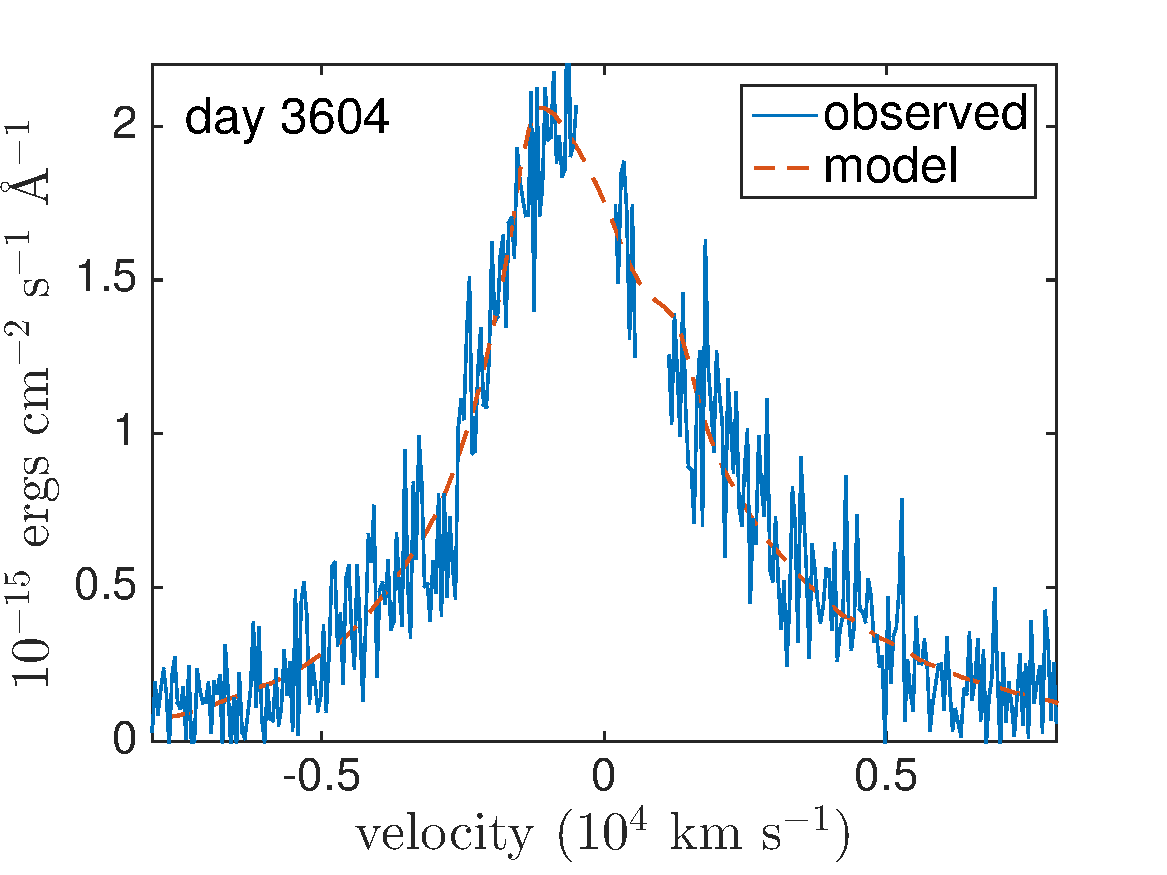
\includegraphics[trim =55 10 45 15,clip=true,scale=0.35]{chapters/chapter5/images/smooth/best_fit/d3604Ha}
\caption{Best smooth fit to the H$\alpha$ line at days 1862, 2875 and 
3604 as per parameters detailed in Table \ref{smooth1}.}
\label{d1862_3604}
\end{center}
\end{figure*}

\subsection{Smooth Density Models for SN 1987A}
\label{smooth_models}

Even at the earliest epochs there is a substantial wing on the red of 
the H$\alpha$ line profile that cannot be fitted by scattering from moving grains with a small albedo.  The 
minimum required albedo is approximately $\omega \approx 0.5$.  The larger 
the grain size the larger the mass of dust required to reproduce the same 
optical depth (since the optical depth is dependent only on the 
cross-sectional area of the grains).  Figure \ref{MRN} illustrates the 
a fit for the day 714 H$\alpha$ profile for the case where a classical MRN grain size 
distribution is adopted, with $a_{min}=0.005 \mu m$, $a_{max}=0.25 \mu m$ 
and $n(a) \propto a^{-3.5}$.  It can be seen clearly that the extended red wing is 
significantly underestimated.  Since the albedo of pure 
amorphous carbon grains varies significantly with grain radius (see Figure \ref{albedo_grain}) we can establish a strong 
lower bound to the mean dust grain radius, which we estimate to be $a \ge 0.35\mu$m.  This is the smallest grain size that is still 
capable of reproducing the red scattering wing at all epochs and we 
therefore use this value throughout our smooth density modelling.

The ejecta inner and outer radii are calculated at each epoch from the maximum 
velocity used, the day number and the specified ratio $R_{in}/R_{out}$.  
The radii generated are consistent with those used in previous models of 
SN 1987A \citep{Ercolano2007, Wesson2015}.  Figures \ref{d714bf} to 
\ref{d1862_3604} show the best fits to the data for days 714 to 3604 whilst 
Table \ref{smooth1} details the parameters used.

It can be seen that, in order to reproduce the blueshifts seen in the 
[O~{\sc i}] $\lambda$6300,6363~\AA\ doublet, considerably larger dust masses 
are required than to fit the H$\alpha$ line.  However, larger maximum 
velocities are also required to fit the wings and a significantly steeper 
density profile is required.  The inner radii remain approximately similar 
in both the H$\alpha$ and [O~{\sc i}] $\lambda$6300,6363~\AA\ models whilst the 
outer radii are significantly different.  This may indicate why a greater 
dust mass is required in order to fit the [O~{\sc i}] doublet; the doublet 
traces the dust to a wider radius than the H$\alpha$ line.


\subsection{Clumped Models for SN 1987A}
\label{clumped_models}


It has been shown through the modelling of optical-IR SEDs that when dust 
is assumed to have a clumped distribution the derived masses can be 
significantly larger than if the dust is distributed smoothly between the 
inner and outer radii.  We present two sets of fits to the line profile based on 
the clumped dust modelling of \citet{Wesson2015}.  Each fit is derived from the best 
fitting smooth model such that the photon packets are emitted assuming a smooth 
radial density profile.  However, the dust is no longer coupled to the gas 
but instead is located entirely in clumps of size $R_{out}/30$.  The 
clumps are distributed stochastically between $R_{in}$ and $R_{out}$ with 
the probability of a given grid cell being a clump proportional to $r^{- 
\beta }$ where $i(r) \propto r^{-2 \beta}$.  The number of clumps used is 
determined by the clump filling factor $f$ which is kept constant at $f=0.1$.  All 
properties are fixed from the smooth models with the exception of the grain 
radius and total dust mass.

As in the case of SED radiative transfer models, the dust masses required to reproduce the 
observations in the clumped case are considerably higher than for the smooth case.  
However, it is also necessary to have a slightly larger albedo in order to 
reproduce the red side of the profiles.  This is because when 
the dust is located in clumps the radiation is subject to less scattering 
as well as to less absorption.  The reduction in scattering appears not to be 
compensated for by the increased dust mass and a larger grain radius is 
therefore required, particularly at day 714.  A grain radius of $a=0.6\mu$m 
is therefore used throughout the clumped models as the smallest possible 
grain size capable of reproducing the observed profiles. Full details of all 
parameters used for these models may be found in Table \ref{clumped1} and 
the fits are presented in Figures \ref{d714_c} to \ref{d1862_3604_c}.


Since these models also utilise the smallest possible grain size and 
therefore represent a minimum dust mass in the case of 
clumped distributions of amorphous carbon grains, we have also investigated the 
potential for this method to derive an upper bound on the dust mass.  By 
steadily reducing the grain size from an initial value of 5$\mu$m 
(motivated by the maximum possible grain size derived by W15 for their day 
8515 model), we produce a set of models representing a theoretical maximal 
dust mass.  Throughout the course of our modelling it transpired that the 
grain size used for the minimum models at days 714 and 806 ($a=0.6\mu$m) 
in fact represents the best fit to the data and even a small fluctuation 
in $a$ in either direction results in a significantly poorer fit, either 
over- or underestimating the red wing and the trough in the doublet.  We 
therefore conclude that the dust mass estimates produced at days 714 and 
806 for a grain radius of $a=0.6\mu$m are the best estimates of the dust mass 
at this epoch.  At later epochs however we find that equally good fits may 
be generated by substantially larger grains, with grain radii up to $a=3.5\mu$m (see Figure 
\ref{d1862_3604_cmax}).  Details of the parameters used in these models 
presented in Table \ref{clumped2}.



\begin{table*}
	\begin{minipage}{180mm}
	\caption{Details of the parameters used for the best fitting clumped models with $a=3.5\mu$m.}
	\label{clumped2}
	\begin{center}
  	\begin{tabular}{@{} ccccccccccl @{}}
    	\hline
  day & $V_{max}$ & $R_{in}/R_{out}$ & $\beta$ & $M_{dust}$ & $a$ & $R_{out}$ & $R_{in}$ & $\tau_{H\alpha}$ & $\tau_V$ & Figure No. \\
	& (km~s$^{-1} $) & & & ($M_{\odot}$) & ($\mu$m) & (cm) & (cm)  \\
	\hline
1862 & 8500 & 0.14 & 1.9 & 2.00E-02 & 3.50 & 1.37E+17 & 1.91E+16 & 0.85 & 1.70 & \ref{d1862_3604_cmax} \\
2875 & 9500 & 0.12 & 2 & 8.00E-02 & 3.50 & 2.36E+17 & 2.83E+16 & 1.15 & 2.30 & \ref{d1862_3604_cmax} \\
3604 & 10250 & 0.12 & 2 & 1.70E-01 & 3.50 & 3.19E+17 & 3.83E+16 & 1.33 & 2.67 & \ref{d1862_3604_cmax} \\
    \hline
  \end{tabular}
  \end{center}
\end{minipage}
\end{table*}


 \begin{figure*}
\begin{center}
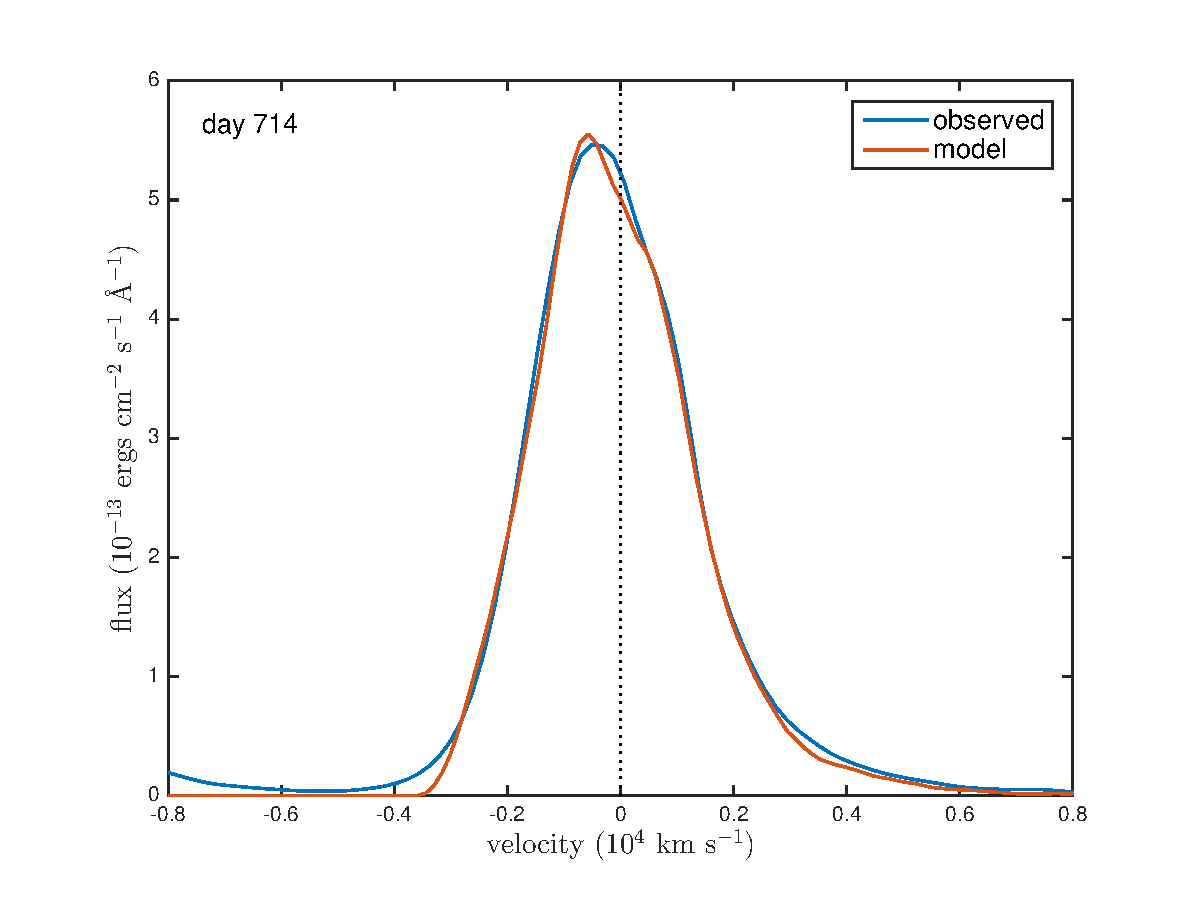
\includegraphics[trim =37 10 45 15,clip=true,scale=0.51]{chapters/chapter5/images/clump_1/best_fit/d714Ha}
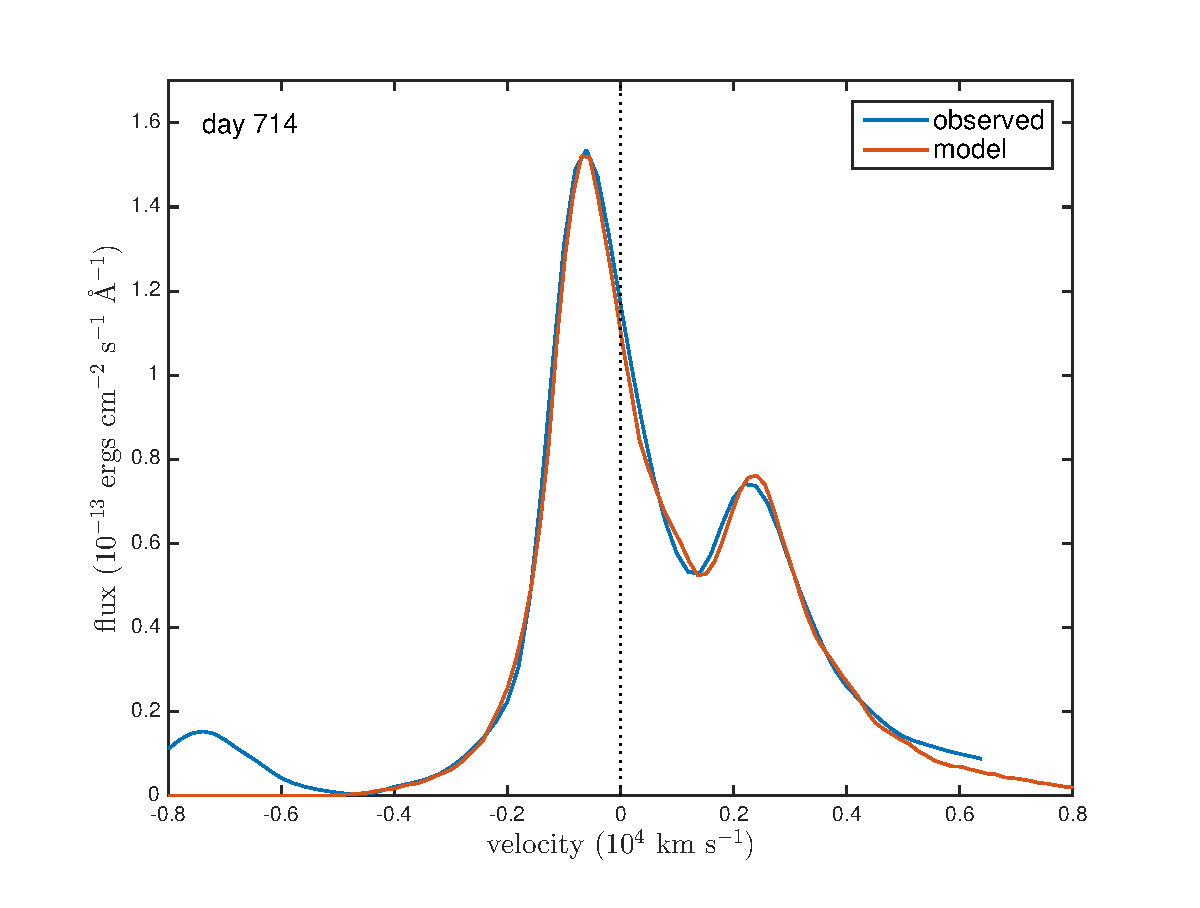
\includegraphics[trim =37 10 45 15,clip=true,scale=0.51]{chapters/chapter5/images/clump_1/best_fit/d714OI}
\caption{Best clumped fit to the day 714 H$\alpha$ line and [O~{\sc i}] 
$\lambda$6300,6363~\AA\ doublet as per parameters detailed in 
Table \ref{clumped1}.}
\label{d714_c}
\end{center}
\end{figure*}
\begin{figure*}
\begin{center}
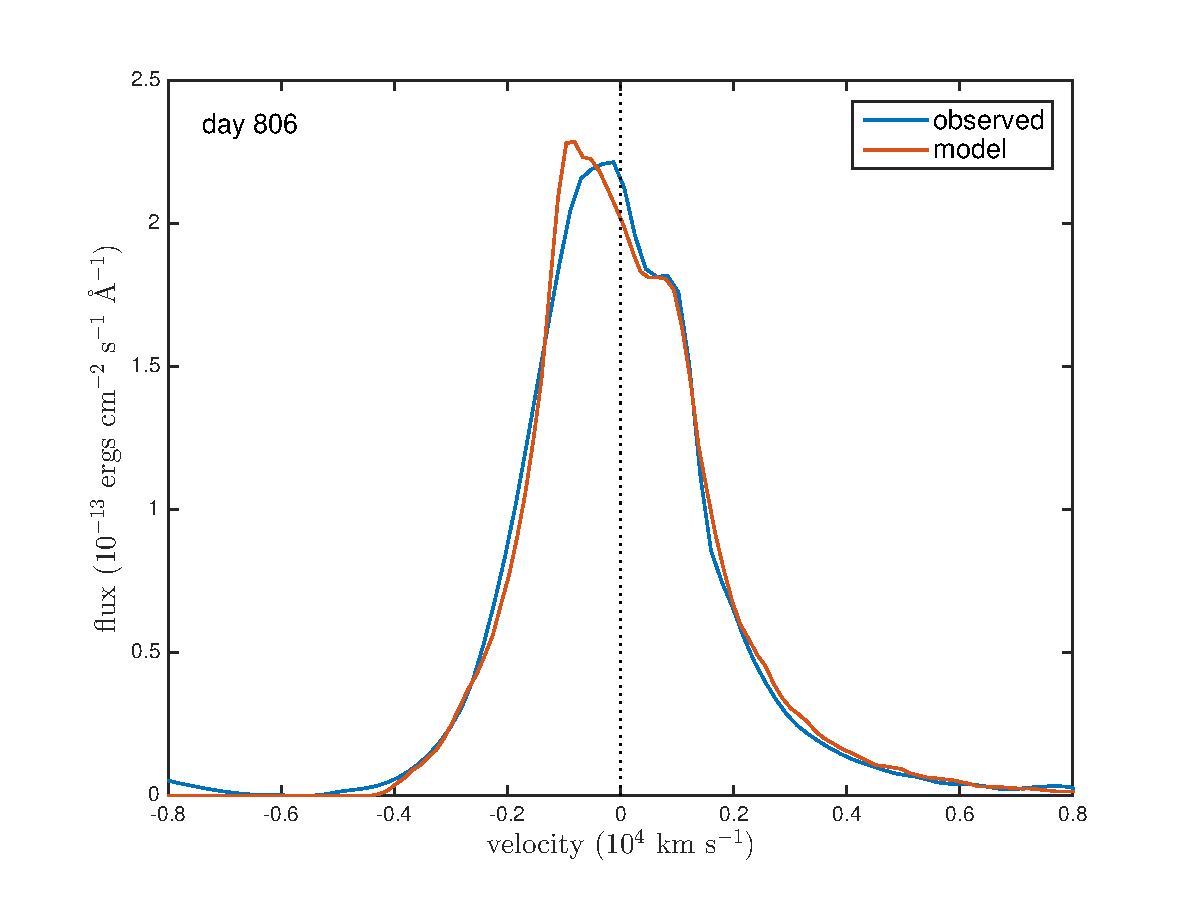
\includegraphics[trim =37 10 45 15,clip=true,scale=0.51]{chapters/chapter5/images/clump_1/best_fit/d806Ha}
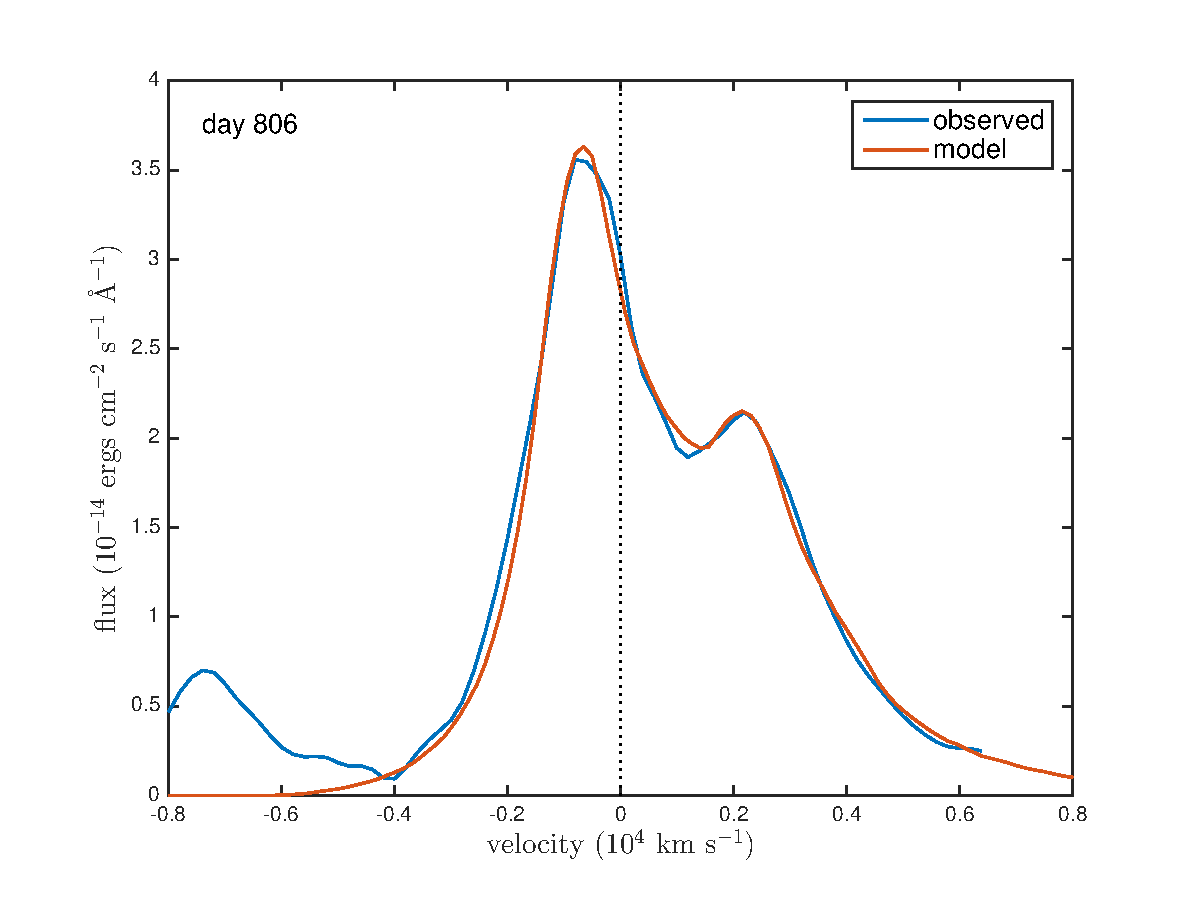
\includegraphics[trim =35 10 45 15,clip=true,scale=0.51]{chapters/chapter5/images/clump_1/best_fit/d806OI}
\caption{Best clumped fit to the day 806 H$\alpha$ line and 
[O~{\sc i}] $\lambda$6300,6363~\AA\ doublet as per parameters detailed in Table 
\ref{clumped1}.}
\label{d806_c}
\end{center}
\end{figure*}

\subsection{Contamination of the the H$\alpha$ profiles at days 714 and 806}

The profile at day 714 (Figure \ref{d714bf}) exhibits several of the features discussed above.  
There is an increase in flux to the red side of $2000$~km~s$^{-1}$ 
as a result of a dust scattering reprocessing radiation to the red.  
There is also an approximately linear section between the peak at $V=-420$ 
km~s$^{-1}$ and the very slight corner visible at $V_{min}$.  The profile 
at day 806 (Figure \ref{d806bf}) has similarly identifiable features with a noticeable wing on 
the red side extending out to nearly $V=8000$ km~s$^{-1}$.  It also exhibits a 
definite shoulder reaching to $V \approx 900$ km~s$^{-1}$ which we assume 
to be the value of $V_{min}$.  In both these cases, with both smooth and 
clumped models, we struggle slightly to fit both the corner and the peak 
of the profile.  In both instances, accurately fitting the corner results 
in a peak that is slightly further towards the blue than is seen in the 
observations.  We suggest that this discrepancy, which is more noticable 
at day 806 because of the more distinctive shape of the profile, is likely 
a result of the increased flux produced by a clump at $V=-360$ 
km~s$^{-1}$.  This clump, clearly visible in the line profile at day 673 
and identified as such in the literature 
\citep{Spyromilio1993a,Hanuschik1993}, is likely contaminating the 
position of the peaks of the profiles at days 714 and 806.  The clump is 
perhaps not so clearly discernible at these epochs as a result of the poor 
resolution of the CTIO spectra but is known to have persisted until around day 
900 \citep{Hanuschik1993}.


\begin{figure*}
\begin{center}
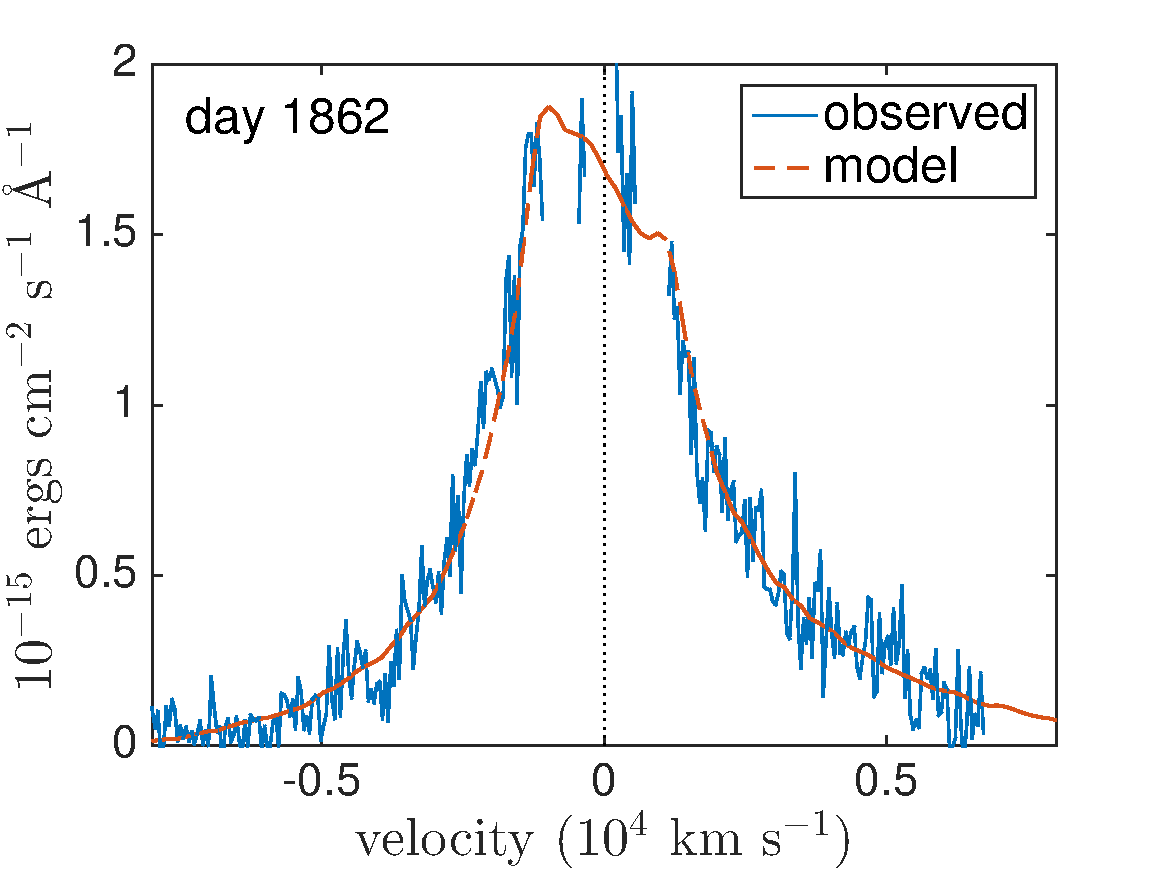
\includegraphics[trim =37 10 45 15,clip=true,scale=0.35]{chapters/chapter5/images/clump_1/best_fit/d1862Ha}
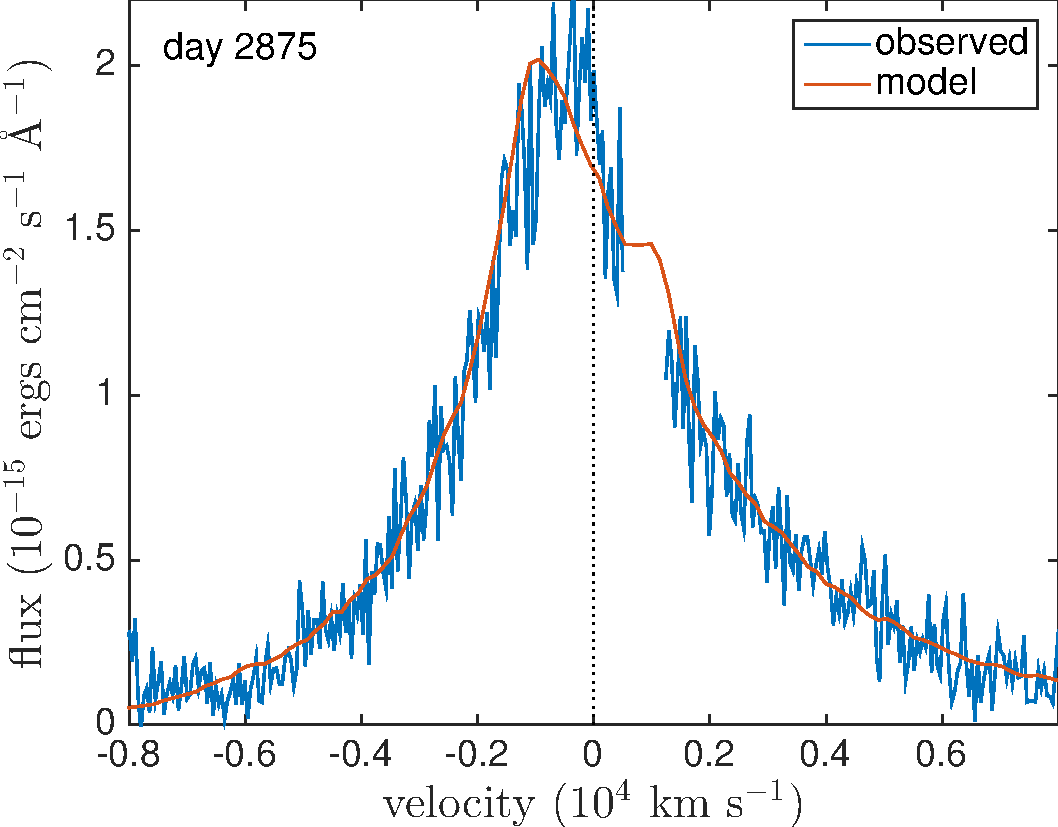
\includegraphics[trim =55 10 45 15,clip=true,scale=0.35]{chapters/chapter5/images/clump_1/best_fit/d2875Ha}
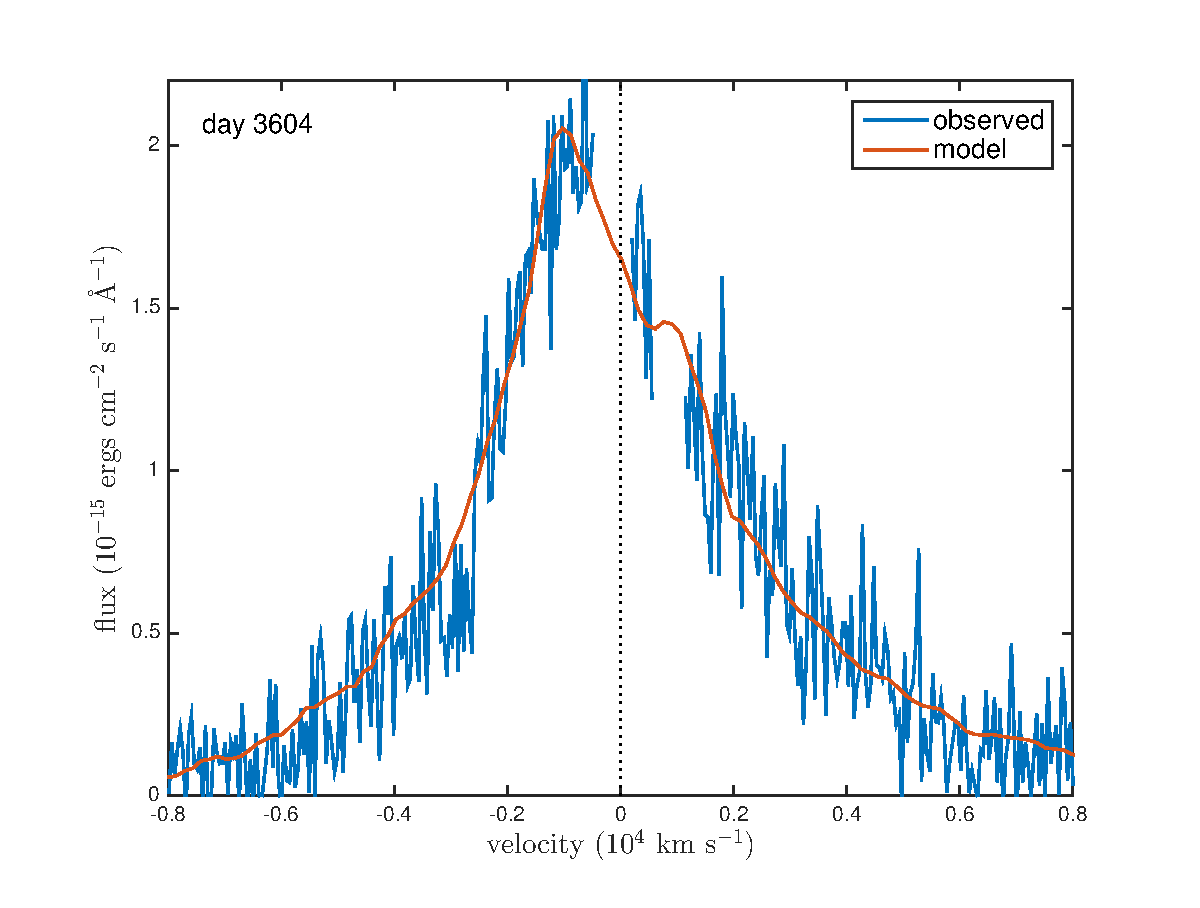
\includegraphics[trim =55 10 45 15,clip=true,scale=0.35]{chapters/chapter5/images/clump_1/best_fit/d3604Ha}
\caption{Best clumped fit to the H$\alpha$ line at days 1862, 2875 and 
3604 as per parameters detailed in Table \ref{clumped1} with $a=0.6\mu$m.}
\label{d1862_3604_c}
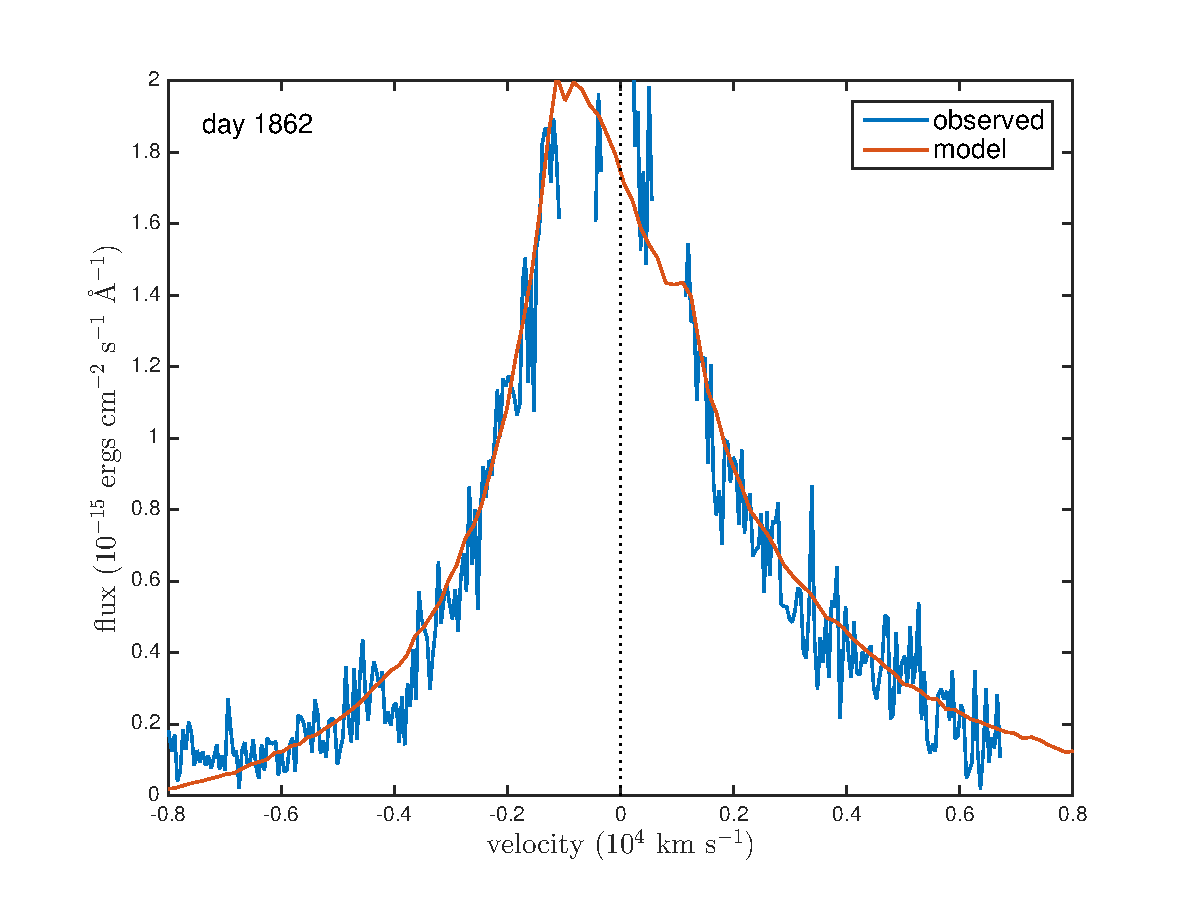
\includegraphics[trim =37 10 45 15,clip=true,scale=0.35]{chapters/chapter5/images/clump_1/maximum/d1862Ha}
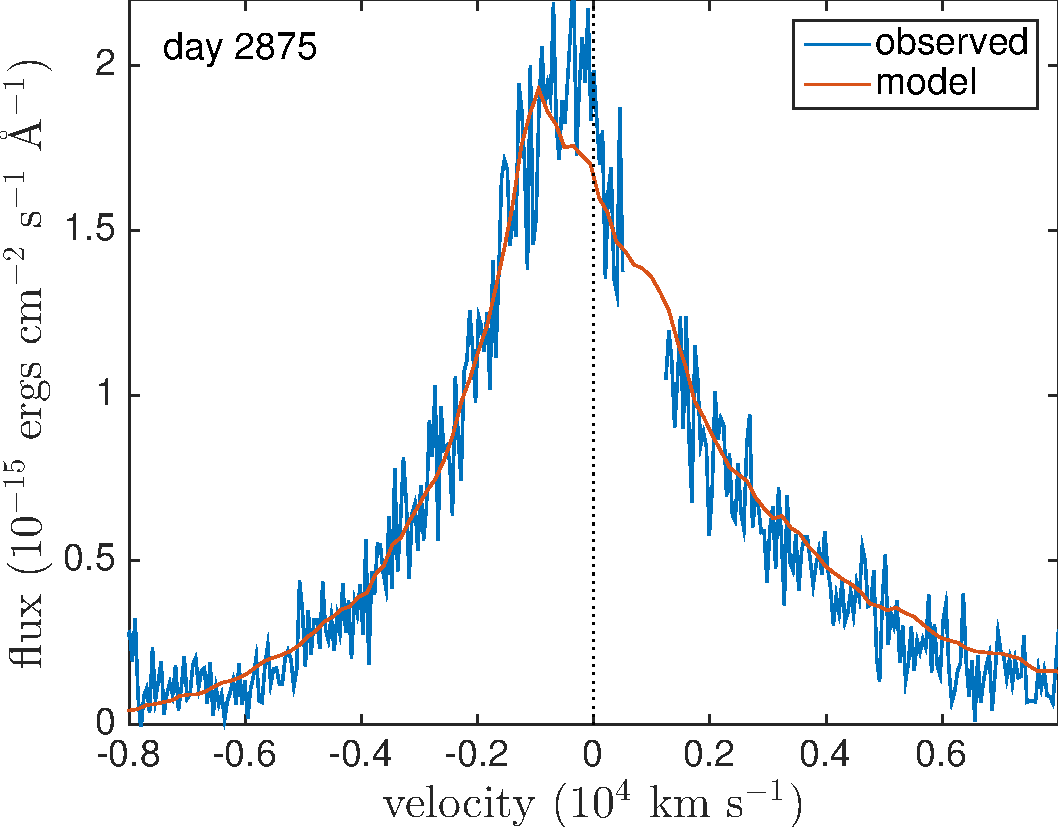
\includegraphics[trim =55 10 45 15,clip=true,scale=0.35]{chapters/chapter5/images/clump_1/maximum/d2875Ha}
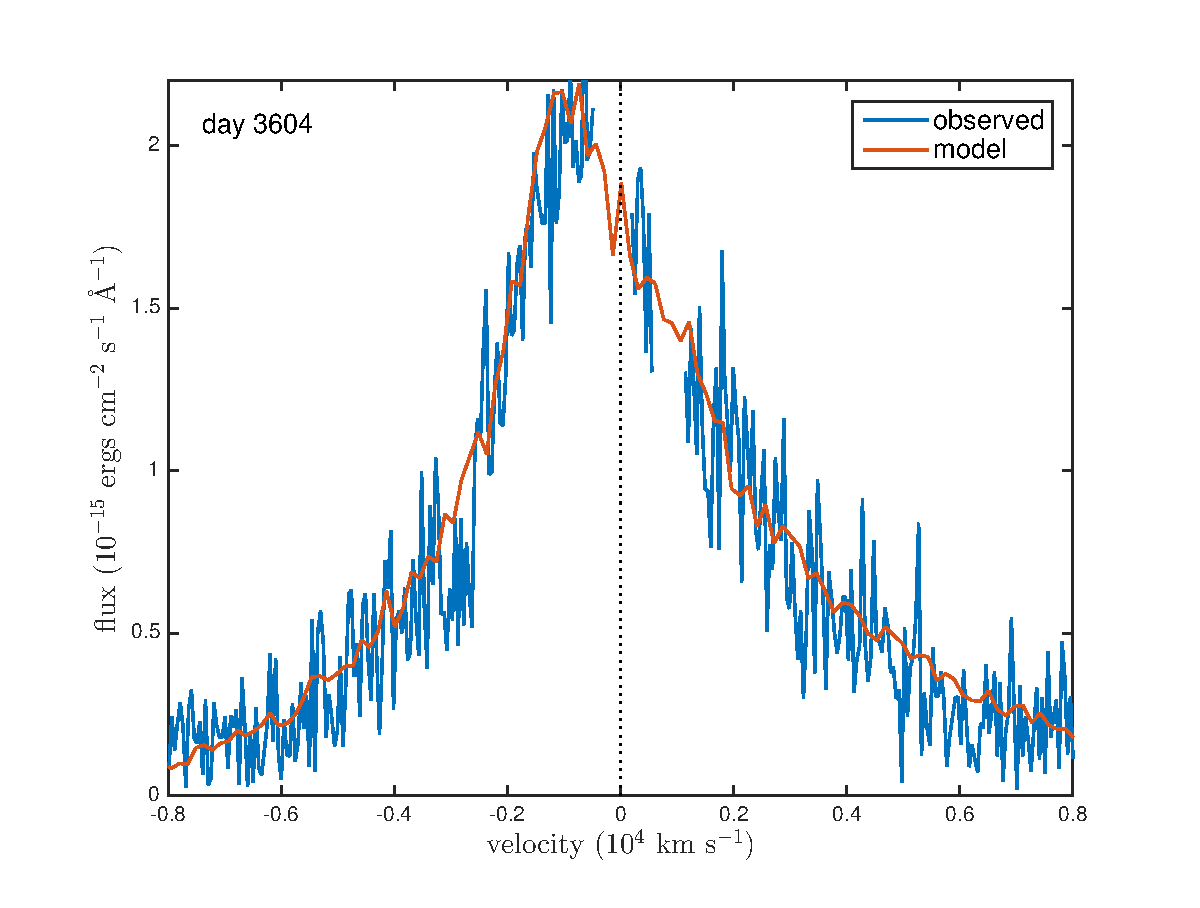
\includegraphics[trim =55 10 45 15,clip=true,scale=0.35]{chapters/chapter5/images/clump_1/maximum/d3604Ha}
\caption{Best clumped fit to the H$\alpha$ line at days 1862, 2875 and 
3604 as per parameters detailed in Table \ref{clumped2} with $a=3.5\mu$m.}
\label{d1862_3604_cmax}
\end{center}
\end{figure*}

\subsection{The red shoulder in the H$\alpha$ line profile at day 806}

The shoulder in the H$\alpha$ line profile at day 806 has previously been 
attributed to an unresolved [NII] $\lambda$6583~\AA\ line at $V=933$ 
km~s$^{-1}$ \citep{Kozma1997}.  Narrow [N~{\sc ii}] lines at $\lambda=$ 
6583~\AA\ and $\lambda=$ 6548~\AA\ either side of the H$\alpha$ rest frame
 velocity at 6563~\AA\ are certainly seen by day 1862 and have to be 
removed in order to consider the evolution of the broad H$\alpha$ profile. 
It is somewhat unfortunate that the theoretical minimum velocity falls at 
a similar velocity to this line as it makes it difficult to distinguish 
the two features.  We postulate however that this feature may in fact be a 
product of a relatively steep density profile and the formation of dust 
within the ejecta as demonstrated in both our fits (see Figures 
\ref{d806bf} and \ref{d806_c}) and our investigation of the parameter 
space (see Figures \ref{bt} and \ref{wt}).

It is a general challenge inherent in the nature of this modelling that 
interesting features that are present in line profiles are not necessarily 
easily identifiable.  In particular, the effects of clumping and 
asymmetrical distributions in the ejecta may cause fluctuations that are 
hard to distinguish from the potential signatures of dust formation 
discussed in Section \ref{params}.  Key indicators such as symmetry in the 
location of discontinuities on the red and blue side, typical dust profile 
signatures and the presence of a red scattering wing should be considered.


\subsection{Potential challenges at later epochs: days 1862, 2875 and 3604}

At later epochs, even very tiny fluctuations in adopted value of the 
continuum level can have a substantial effect on the fit of the resulting 
profile.  Since it is not feasible to establish the level of the continuum 
so precisely, the value of the continuum has been left as a free parameter 
that may be adjusted (to within sensible margins) in order to allow for 
the widest possible dust mass range to be determined.  We generally find 
it is necessary to assume a continuum level that is slightly lower where 
the adopted dust mass is higher.

The line profiles at these later epochs are relatively noisy and have had 
substantial sections of the profile removed as a result of contamination 
by the H$\alpha$ and [NII] narrow lines.  Unfortunately, this removes a 
critical section of the line ($500$ km~s$^{-1}<v<1500$ km~s$^{-1}$) that 
would be potentially informative about $V_{min}$.  However, we do achieve good fits 
to the line profiles at these epochs.



\section{The evolution of dust formation in SN~1987A}
\label{discuss}


We have collated a range of archival spectral data in the optical and IR 
and, by modelling the evolution of the H$\alpha$ and 
[O~{\sc i}] $\lambda$6300,6363~\AA\ lines, have placed constraints on the 
evolution of newly formed dust in SN 1987A. We have done this using Monte Carlo 
models that consider both the absorbing and scattering effects of dust.  
We find dust masses that are in good agreement with those previously 
found at similar epochs.  We obtain large dust masses at just a few 
thousand days in agreement with the very large mass of dust deduced by from their observations at long wavelengths 
using Herschel \citep{Matsuura2011}. We compare our dust masses directly with those obtained by 
W15 and by \citet{Lucy1989b} in order to compare both their magnitude and evolution (see Figure 
\ref{Mdust}).

\subsection{Dust masses from other line profile models}

\citet{Lucy1989b} analysed the [O~{\sc i}]$\lambda$6300~\AA\ line for SN~1987A and found optical depths for a range of epochs. They translated these into dust masses for day 775 only.  
For our smooth modelling of [O~{\sc i}] we obtain $\tau_V=2.19$ at day 714 and $\tau_V=1.95$ at day 806.  These values are somewhat higher than the values given by \citet{Lucy1989b} at similar epochs.  At day 725, they cited a value of $\tau_V=1.19$ and at day 775 a value of $\tau_V=1.25$.  The primary reason for the discrepancy in these values is the assumed albedo.  \citet{Lucy1989b} considered line profiles before and after dust condensation and concluded that any evidence of an extended red scattering wing was unconvinving.  Accordingly, they adopted a model with perfectly absorbing dust ($\omega = 0$).  For our amorphous carbon models of [O~{\sc i}]$\lambda$6300,6363~\AA\ with grain radius $a=0.35\mu$m, we obtain an albedo of approximately $\omega = 0.5$ at $\lambda=6300$ \AA.  The total optical depth to absorption is therefore very similar comparing our model at day 714 to their results at day  725.  There is slightly more discrepancy between our model at day 806 and their model at day 775.  


However, \citet{Lucy1989b} noted that the dust optical depth increased rapidly after day 580 and then the rate of increase of the dust optical depth appeared to slow after day 670.  Our results, for both clumped and smooth models, suggest that the dust optical depth actually drops between day 714 and day 806 before starting to increase again at later epochs.  This is consistent with the results of \citet{Lucy1989b} where the slowing rate of increase of dust optical depth could imply an impending turning point subsequent to day 775.  If a turnover did in fact occur at this time then it could explain the difference in our values.

Finally, the dust masses derived by \citet{Lucy1989b} at day 775 ($M_{dust}=4.4 \times 10^{-6} M_{\odot}$ for amorphous carbon) are significantly different to those obtained from our smooth modelling of the [O~{\sc i}]$\lambda$6300,6363~\AA\ doublet at day 806 ($M_{dust}=1.6 \times 10^{-4} M_{\odot}$ for amorphous carbon).  There are three main reasons for the discrepancy.  Firstly, the albedo is significantly larger in our modelling as already discussed so a larger dust mass is required to produce the same amount of absorption.  Secondly, the grain size is considerably larger which reduces the total cross-section of interaction, and finally, the adopted maximum velocity (6000~km~s$^{-1}$) in our model is larger than the value adopted by \citet{Lucy1989b} (1870~km~s$^{-1}$).  This increases the total volume of the ejecta significantly and therefore significantly more dust is required to produce the same optical depth.

\subsection{Dust masses and properties from SED models}

Considering now the results of W15, we find that at all epochs we obtain slightly smaller dust masses than those of W15 although our values are still generally within the error bars 
placed on their values.  There may be a number of different reasons for 
this.  Firstly, our modelling is somewhat more conservative in its 
estimates since we use amorphous carbon whereas the 
models presented by W15 use a silicate fraction of 15\% which is likely to 
increase the overall mass of dust required to produce the same 
observations, both in the case of radiative transfer SED modelling and 
line profile modelling.  Secondly, we use different sets of optical 
constants; we have used the optical constants derived by \cite{Zubko1996} 
from their BE sample where W15 use constants from 
\cite{Hanner1988}.  They state that in order to 
fit their data at early epochs (day 615) with the Zubko ACH2 sample 
smaller inner and outer radii are needed and half as much dust ($5.0 
\times 10^{-4}M_{\odot}$) is required.  This is considerably closer to the 
values we derive at similar epochs.


\begin{figure*}
\begin{center}
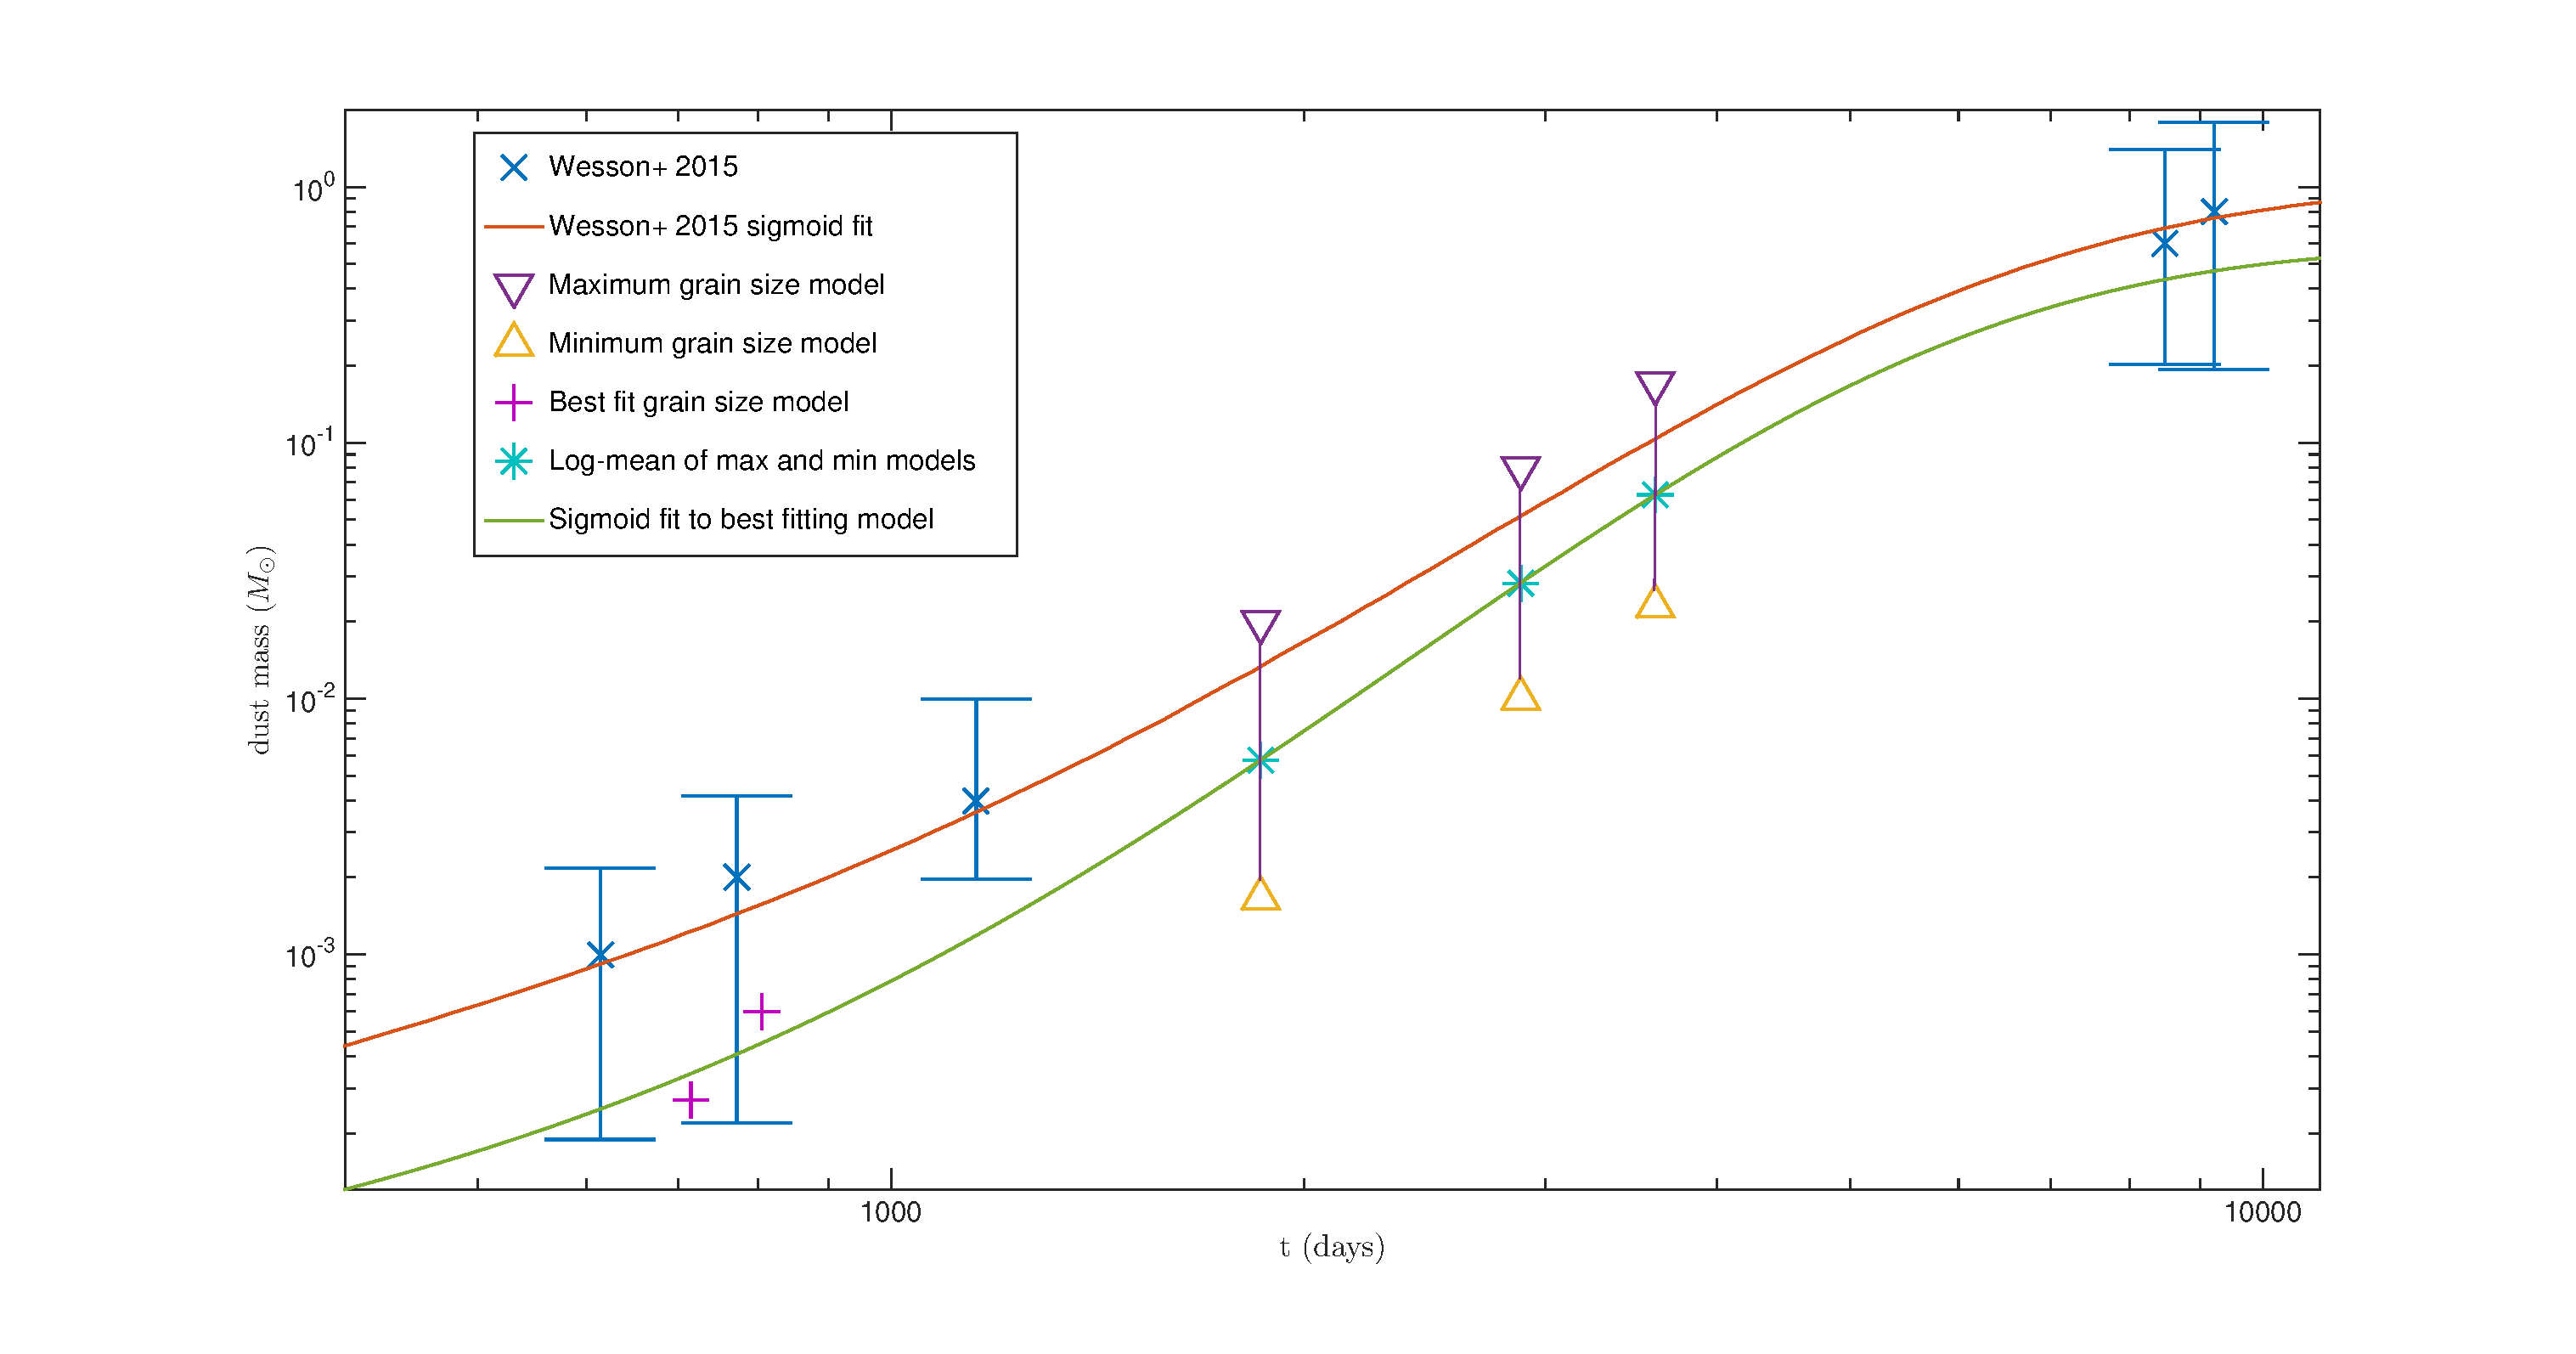
\includegraphics[trim =120 30 105 15,clip=true,scale=0.41]{chapters/chapter5/images/Mdust_evol2}
\caption{\textit{Purple and yellow triangles -} Maximum ($a=3.5\mu$m) and 
minimum ($a=0.6\mu$m) dust masses respectively.  Values are from the 
later epoch ($t>1862$ days) clumped models of H$\alpha$.  \textit{Pink 
crosses - } Predicted dust masses (clumped models of the 
[O~{\sc i}] $\lambda$6300,6363~\AA\ doublet with grain size $a=0.6\mu$m).  
\textit{Turquoise stars -} Predicted dust masses calculated as a log 
average of the maximum and minimum values.  \textit{Green -} Sigmoid fit 
to our predicted dust masses. \textit{Blue - } dust masses derived by W15 
in their photometric modelling of SN 1987A. \textit{Red} - sigmoid fit to 
the W15 values.}
\label{Mdust}
\end{center}
\end{figure*}

The other significant difference between our models is the adopted grain 
size distribution.  W15 generate fits to their ealy data using an MRN 
distribution between 0.005$\mu$m and 0.25$\mu$m in size.  They cannot 
obtain a fit with grains of $\sim 1.0 \mu$m in size at early epochs.  
However, they do not consider values in between these size point as we 
conclude is likely the case with grain sizes of $a \approx 0.6\mu$m.  For 
SED modelling it is generally the case that the larger the grain size 
used, the less dust is required to produce the same level of flux and it 
may therefore be this difference that is generating the discrepancy in our 
results.  W15 use this property to derive a maximum possible grain size at 
late epochs as well and conclude that grains cannot be larger than $\sim 
5\mu$m by day 8515.  This is directly in line with the maximum grain sizes 
we derive at slightly earlier epochs.  We find that the grain size likely 
cannot have exceeded $\sim 3.5\mu$m at day 3604 and the dust masses that 
we generate using this value are very similar to the value of the W15 
sigmoid fit at this epoch.


Determining the relationship between the size of dust grains in the ejecta 
and the time post-explosion is important for understanding the likelihood 
of dust surviving the passage of the reverse shock travelling back through 
the ejecta. By the time the reverse shock begins to appear in the line 
profiles (around day 5000), our models predict that the grains could 
already be as large as several microns in radius but are certainly larger 
than $\sim 0.6\mu$m.  Grains larger than $\sim 0.2\mu$m are likely to 
survive and thus the majority of the dust produced is likely to survive 
(remembering that our modelling only considers an average grain size and 
makes no comment about the grain size distribution).  It has recently been 
suggested that very large grains (up to 4.2$\mu$m) may have formed in the 
ejecta of SN 2010jl very soon after the explosion (a few hundred days) 
\cite{Gall2014}.  Whilst the values we suggest are not as high that 
postulated by \citet{Gall2014}, they maintain a distribution that remains 
steeped towards the smaller end of the scale and thus, as our models only 
treat a single, average grain size, these values may be not be at odds.  
Certainly, both results suggest that grains large enough to survive the 
destructive force of the reverse shock have formed by a few hundred days 
post-explosion.

There is now a firm consensus that a very large quantity of dust has 
formed in SN 1987A between the time of the original explosion and the 
present day.  Perhaps more important therefore is the manner of its 
evolution.  We have shown that dust masses have reached the order of 
$0.1M_{\odot}$ by day 3604.  However, it is known that values several 
times as large as this are ultimately expected and thus a substantial 
fraction of the dust is likely to form after this epoch.  This is in 
strong agreement with the results produced by W15.  They derive a sigmoid 
fit to their dust mass evolution of the form

\begin{equation}
M_d(t)=ae^{be^{ct}}
\end{equation}
 
where they obtain values of $a=1.0M_{\odot}$ (representing the maximum 
dust mass), $b=-8.53$ and $c=-0.000366$.  Both their dust masses and this 
sigmoid fit are shown in Figure \ref{Mdust}.  This exhibits an initial 
period of slow growth followed by an intermediary period of acceleration 
followed by another slowing until a plateau is ultimately reached.  In 
this sense it may be relatively representative of the process of dust 
formation whereby initial conditions appropriate for grain growth 
gradually develop until optimal conditions are reached at an intermediate 
epoch when grain growth is at its fastest before conditions once again 
deteriorate and the rate slows again (as discussed by W15).  Performing a 
least-squares regression to this function using our predicted dust masses, 
we derive a sigmoid fit with coefficients $a=0.58M_{\odot}$, $b=-10.02$ 
and $c=-0.000416$.  These values are remarkably similar to those derived 
by W15 although the final predicted dust mass is slightly smaller in our 
case.  This sigmoid fit is also plotted in Figure \ref{Mdust}.

Our modelling concurs with the suggestion of W15 that even after 
$\sim$3000 days the dust mass is only a very small fraction of its final 
value.  This is in contrast to \citet{Sarangi2015} whose chemistry models 
predict that the evolution of dust formation will have reached its plateau 
by around 5 years after the explosion first occured.

Ideally, our models would cover the entire evolution of SN 1987A right up 
to the present day.  However, the excitation of gas in the outer edges of 
the ejecta by the reverse shock after $\sim$ day 500 results in a 
significant, broad and asymmetric flux that dominates the original line 
profile.  In addition to this, the narrow lines from the ring start to 
become so significant relative to the original broad H$\alpha$ profile 
that, post-removal, there is not enough of the broad profile remaining to 
be able reliably infer information from its features.  These are factors 
that are likely to be common to most core collapse supernovae and thus are 
likely to have an impact on the wider applicability of this particular 
technique at later epochs.  Care should also be taken in the future to 
ensure that the line profiles are the temporally appropriate profile and 
not in fact a product of a light echo representing the state of the ejecta 
at some previous epoch.  Nonetheless, this technique has proved effective 
in determining dust masses formed in core-collapse supernovae through the 
detailed modelling of asymmetric line profiles and clearly has wider 
application to multiple supernovae and supernova remnants.



